
\documentclass{jsreport}
\usepackage[utf8]{inputenc}
\usepackage[dvipdfmx,colorlinks=true, bookmarks=true,bookmarksnumbered=true, bookmarkstype=toc, linkcolor=cyan,urlcolor=cyan, citecolor=cyan]{hyperref}
\usepackage{pxjahyper}
\usepackage[dvipdfmx]{graphicx}
\usepackage[dvipdfmx]{color}
\usepackage{multirow}
\usepackage{here}
\usepackage{amsmath}
\usepackage{float}
\usepackage{url}
\usepackage{setspace}


% ユーザー変数
\newcommand{\myname}{中村 竜也}
\newcommand{\studentid}{211S114S}
\newcommand{\submitdate}{令和5年2月 日}
\newcommand{\papertitle}{LHC-ATLAS実験Run-3に向けた\\???}

\newcommand{\ctext}[1]{\raise0.2ex\hbox{\textcircled{\scriptsize{#1}}}} %丸文字を\ctext{}で入力できるようにする
\newcommand{\unit}[1]{\ \mathrm{#1}} %\unit{}で単位を入力できるようにする。
\newcommand{\siki}[1]{式(\ref{#1})} %式の参照を楽に
\newcommand{\zu}[1]{図\ref{#1}} %図の参照を楽に
\newcommand{\hyou}[1]{表\ref{#1}} %表の参照を楽に
\newcommand{\setu}[1]{\ref{#1}節}
\newcommand{\syou}[1]{第\ref{#1}章}
\newcommand{\pt}{p_\mathrm{T}}

\makeatletter %数式,図,表番号に章番号も含む
\@addtoreset{equation}{chapter}
\def\theequation{\thechapter.\arabic{equation}}
\@addtoreset{figure}{chapter}
\def\thefigure{\thechapter.\arabic{figure}}
\@addtoreset{table}{chapter}
\def\thetable{\thechapter.\arabic{table}}
\makeatother




\begin{document}
\addtocounter{page}{-3}
\thispagestyle{empty}

\vspace*{1.5cm}

\begin{center}
  \begin{huge}
    修  士  学  位  論  文
  \end{huge}

  \vspace{2cm}

  \begin{huge}
    \begin{spacing}{1.1}
      \fontsize{19pt}{20pt}\selectfont
      \papertitle
    \end{spacing}
  \end{huge}
  
  \vspace{3cm}

  \begin{LARGE}
    \begin{spacing}{1.1}
        \flushright \submitdate\\
        \vspace{1cm}
        \begin{center}
            専\hspace{2.2mm}攻\hspace{2.2mm}名\hspace{4.5mm}物理学専攻\\
            \hspace{-2.2mm}学籍番号\hspace{4.5mm}\studentid\\
            氏  名\hspace{4.5mm}\myname\hspace*{2.2mm}
        \end{center}
    \end{spacing}
  \end{LARGE}

  \vspace{4.0cm}

  \begin{LARGE}
    \fontsize{17pt}{20pt}\selectfont
    神戸大学大学院理学研究科博士課程前期課程
  \end{LARGE}
\end{center}
\begin{comment}

\newpage
~
\thispagestyle{empty}
\newpage
\thispagestyle{empty}
\newpage
%\linenumbers

%----abstract----
\begin{center}
\begin{huge}
概要
\end{huge}
\end{center}

\vspace{10pt}

Large~Hadron~Collider~(LHC)は、欧州原子核研究機構~(CERN)に建設された世界最高エネルギーの陽子陽子衝突型加速器である。ATLAS検出器は、LHCの衝突点の1つに設置された大型汎用検出器であり、TeVエネルギー領域の陽子衝突で生成される粒子を測定することで、新粒子の直接探索やヒッグス粒子の精密測定を行い、素粒子標準模型を超えた新物理の発見を目指している。

LHCにおける陽子陽子衝突は高頻度であるため、すべての衝突事象を記録することはできない。そのためトリガーシステムを使用し、物理として興味のある事象のみを選別し保存している。
LHC及びATLAS検出器は2019年から2022年までの期間にアップグレードが行われ、2022年7月から重心系エネルギー13.6~TeVでの第三期運転~(Run-3)として実験が行われている。

ルミノシティの増加に伴って事象数も増加するため、物理事象の選別を行うトリガーシステムの改良が必要不可欠である。
トリガーシステムの中でも初段トリガーに分類されるエンドキャプ部の初段ミューオントリガーは、Thin-Gap~Chambers~(TGC)というミューオン検出器を用いて横方向運動量を指針としたトリガー判定を行っている。このとき、ミューオンの飛跡の曲がり具合と横方向運動量の対応を関連づけたCoincidence~Window~(CW)と呼ばれる参照表を用いることで、短時間で飛跡情報からミューオンの横方向運動量を算出している。

初段ミューオントリガーのトリガー性能の改善に向けて、CWをRun-3に対応したものに作り直す必要がある。
CWはシミュレーションデータから作成しているため、実際の検出器のズレや歪みが考慮されておらず、そのまま実際の測定に使用するとトリガー性能が低下してしまう。
そこで、検出器のズレや歪みに対する補正を行うことでCWを最適化し、トリガー性能を向上させる手法が先行研究によって確立されてきた。
しかし、従来の手法ではCWの作成の手間の多さや手動で行う最適化の作業量が膨大であることが問題となり、従来の手法に代わる効率的なCWの作成及び最適化手法が求められた。そこで、機械学習を用いて効率的にCWを作成し最適化を行う手法の開発を行う。

本研究では、実際の実験データを機械学習のトレーニングに使用することで、自動的に検出器のズレや歪みに対する補正を行うことのできる手法の開発を行い、CW作成の効率化を図った。また、作成したCWを用いた際のトリガー性能について、従来の手法で作成したCWと比較を行い、本研究の手法によってトリガー性能を向上させることが可能であることを示した。本発表では、開発したCWの作成手法と、作成したCWのトリガー性能の評価について述べる。
\newpage
\thispagestyle{empty}
%\newpage

%----table----
\pagenumbering{roman}
\setcounter{tocdepth}{2} %目次:subsectionまで表示
\tableofcontents
\newpage

%----document----
\pagenumbering{arabic}
%\newpage

\chapter{序論}
我々の身の回りにある物質を構成する最小単位は素粒子である。
この物質の最小単位である素粒子と、素粒子の相互作用を記述した理論として標準模型が存在している。素粒子物理学において、自然界には電磁相互作用、強い相互作用、弱い相互作用、重力相互作用といった4種類の基本相互作用が存在すると考えられており、標準模型では重力相互作用以外の3種類の相互作用が記述されている。
標準模型は、12種類のフェルミオン、4種類のゲージボソン、ヒッグス粒子の計17種類の粒子から構成されている。
2012年にヒッグス粒子がATLAS実験とCMS実験によって実験的に発見されたことによって、標準模型は。
しかし、標準模型には多くの未解決問題が残されている、この問題を解決するためには、標準模型を超える新しい物理が必要であり、新しい物理を探索するための実験が世界中で行われている。



\chapter{LHC-ATLAS実験}
\label{chapter2}

LHC-ATLAS 実験とは、LHC (Large Hadron Collider)を用いた高エネルギーの陽子–陽子衝突によって生成された粒子を ATLAS (A Troidal LHC ApparatuS) 検出器によって検出し、標準模型の精密測定や新粒子探索などを行う実験である。
LHCでは高エネルギー状態の陽子を衝突させることにより、TeV スケールまでの物理事象を広く調べることを可能にしている。
LHC は 2018 年に Run-2 を終了し、2019 年から 2021 年にかけて LHC 及び ATLAS 検出器のアップグレードが行われ、2022 年から Run-3 が開始された。

本章では、Run-3におけるLHC及びATLAS検出器の概要とATLAS実験で採用されているトリガーシステムについて述べる。

\section{LHC加速器}
\label{section2-1}
Large Hadron Collider (LHC)は、スイスのジュネーブ郊外にある欧州素粒子原子核研究機構 (CERN)の地下に建設された周長約 27 km の世界最大の大型ハドロン衝突型加速器である。LHCの全体像を図\ref{fig:LHC加速器}に示す。
LHC は14 TeV の重心系エネルギー、$1\times10^{34}$ cm$^{-2}$s${^-1}$の瞬間ルミノシティで陽子-陽子衝突が可能なように設計されている。LHCの衝突実験で使用される陽子ビームはバンチと呼ばれる 10${^11}$ 個の陽子のかたまりで構成されており、LHCの一周あたりに 25 ns のバンチ間隔で入射されているため、陽子-陽子衝突を起こす際の各バンチの衝突頻度は 40 MHz となっている。
Run-3では陽子-陽子衝突の重心系エネルギーを 13.6 TeVに増強し、瞬間ルミノシティ 2.0$\times$10$^{34}$ cm$^{−2}$s$^{−1}$ での運転を行い、Run-2 で取得したデータと合わせて積分ルミノシティで 350 fb$^{−1}$ のデータを取得する予定である。

\begin{figure}[tb]
  \centering
  \includegraphics[clip]{fig/2/accel_complex-v2022_complex.png}
  \caption{LHC加速器の概略図}
  \label{fig:LHC加速器}
\end{figure}


LHCでは陽子を衝突させる前に、いくつかの前段加速器を使用しTeVスケールの高エネルギーまで加速している。
初めに水素原子に強い電場をかけることで、衝突実験で使用する陽子を得る。
この陽子は線形加速器である LINAC2 で 50MeV まで加速される。次に、Proton Synchrotron Booster (PSB) で1.4GeVまで加速された後、Proton Synchrotron (PS) で陽子を26GeVまで加速し、40MHzのバンチ構造を持った陽子ビームを形成する。
その後、Super Proton Synchrotron (SPS) で450GeVまで加速された後、陽子ビームはLHCに入射され最大で7 TeV まで加速される。
LHCは陽子ビームが反対方向に周回するための2つのリングから構成されており、4か所ある衝突点にそれぞれ検出器が設置されている。
その衝突点の一つに ATLAS 検出器が設置され、陽子同士の衝突から生成される粒子を検出する。
他3箇所にも検出器が設置されており、それぞれCMS(Compact Muon Solenoid)、LHCb (Large Hadron Collider b)、ALICE (A Large Ion Collider Experiment)である。
ATLAS と CMS の2つの検出器は、標準模型の検証から標準模型を超える現象の探索まで可能な汎用検出器である。
LHCb と呼ばれる検出器は、B-ハドロン系の物理を研究するために設計されたものである。
最後の ALICE は、QCD 現象を探るために重イオン衝突の研究に最適化された検出器である。

\section{LHC-ATLAS 実験}
\label{section2-2}
本節では、LHC-ATLAS 実験で使用される ATLAS 検出器とトリガーシステムについて説明する。

\subsection{ATLAS検出器}
ATLAS検出器は、LHCの衝突点の1つに設置された、直径25m、長さ44mの円筒形の大型汎用検出器である。全体像を図\ref{fig:ATLAS検出器}に示す。
ATLAS検出器は複数の検出器を組み合わせて構成されており、内側から大きく分けて内部飛跡検出器、カロリメータ、ミューオン検出器といった検出器が設置されている。また、内部飛跡検出器とカロリメータの間には超電導ソレノイド磁石、カロリメータの外側にはトロイド磁石がそれぞれ設置されている。
これらの検出器から得られる情報を組み合わせることで、粒子識別や粒子のエネルギーなどの測定を行っている。
以下では各検出器の概要について述べる。

\begin{figure}[tb]
  \centering
  \includegraphics[clip,width=14cm]{fig/2/0803012_01.jpg}
  \caption{ATLAS検出器の全体図}
  \label{fig:ATLAS検出器}
\end{figure}


\subsection{ATLAS検出器における座標系}
ATLAS実験では図\ref{fig:a}に示すような直行座標系と円筒座標系が使用されている。直行座標系では、検出器の中心を原点として、ビーム軸に沿ってz軸を取る。ビーム軸に垂直な平面をx-y平面としたときに、加速器の中心方向を正とするx軸及び、地面に対して垂直方向上向きを正とするy軸を設定する。円筒座標系では、ビーム軸に沿ったz軸に対し、動径方向を$R$、ビーム軸周りの角度を方位角$\phi$、ビーム軸からの角度を極角$\theta$としている。
ATLAS 検出器では z 軸が正の側を A-side、負の側を C-side と定義している。

また、ATLAS実験で使用される座標系として、
\begin{equation}
 \eta=-ln(tan\frac{\theta}{2})
 \label{ラピディティ}
\end{equation}

と定義される擬ラピディティ$\eta$が用いられる。

ATLAS 検出器は円筒形をしており、側面部分と底面部分に配置される検出器を分けて考えるため、$|\eta| < 1.0$ の側面部分をバレル領域、$|\eta| > 1.0$ の底面部分をエンドキャップ領域と呼ぶ。



\begin{figure}[tb]
  \centering
  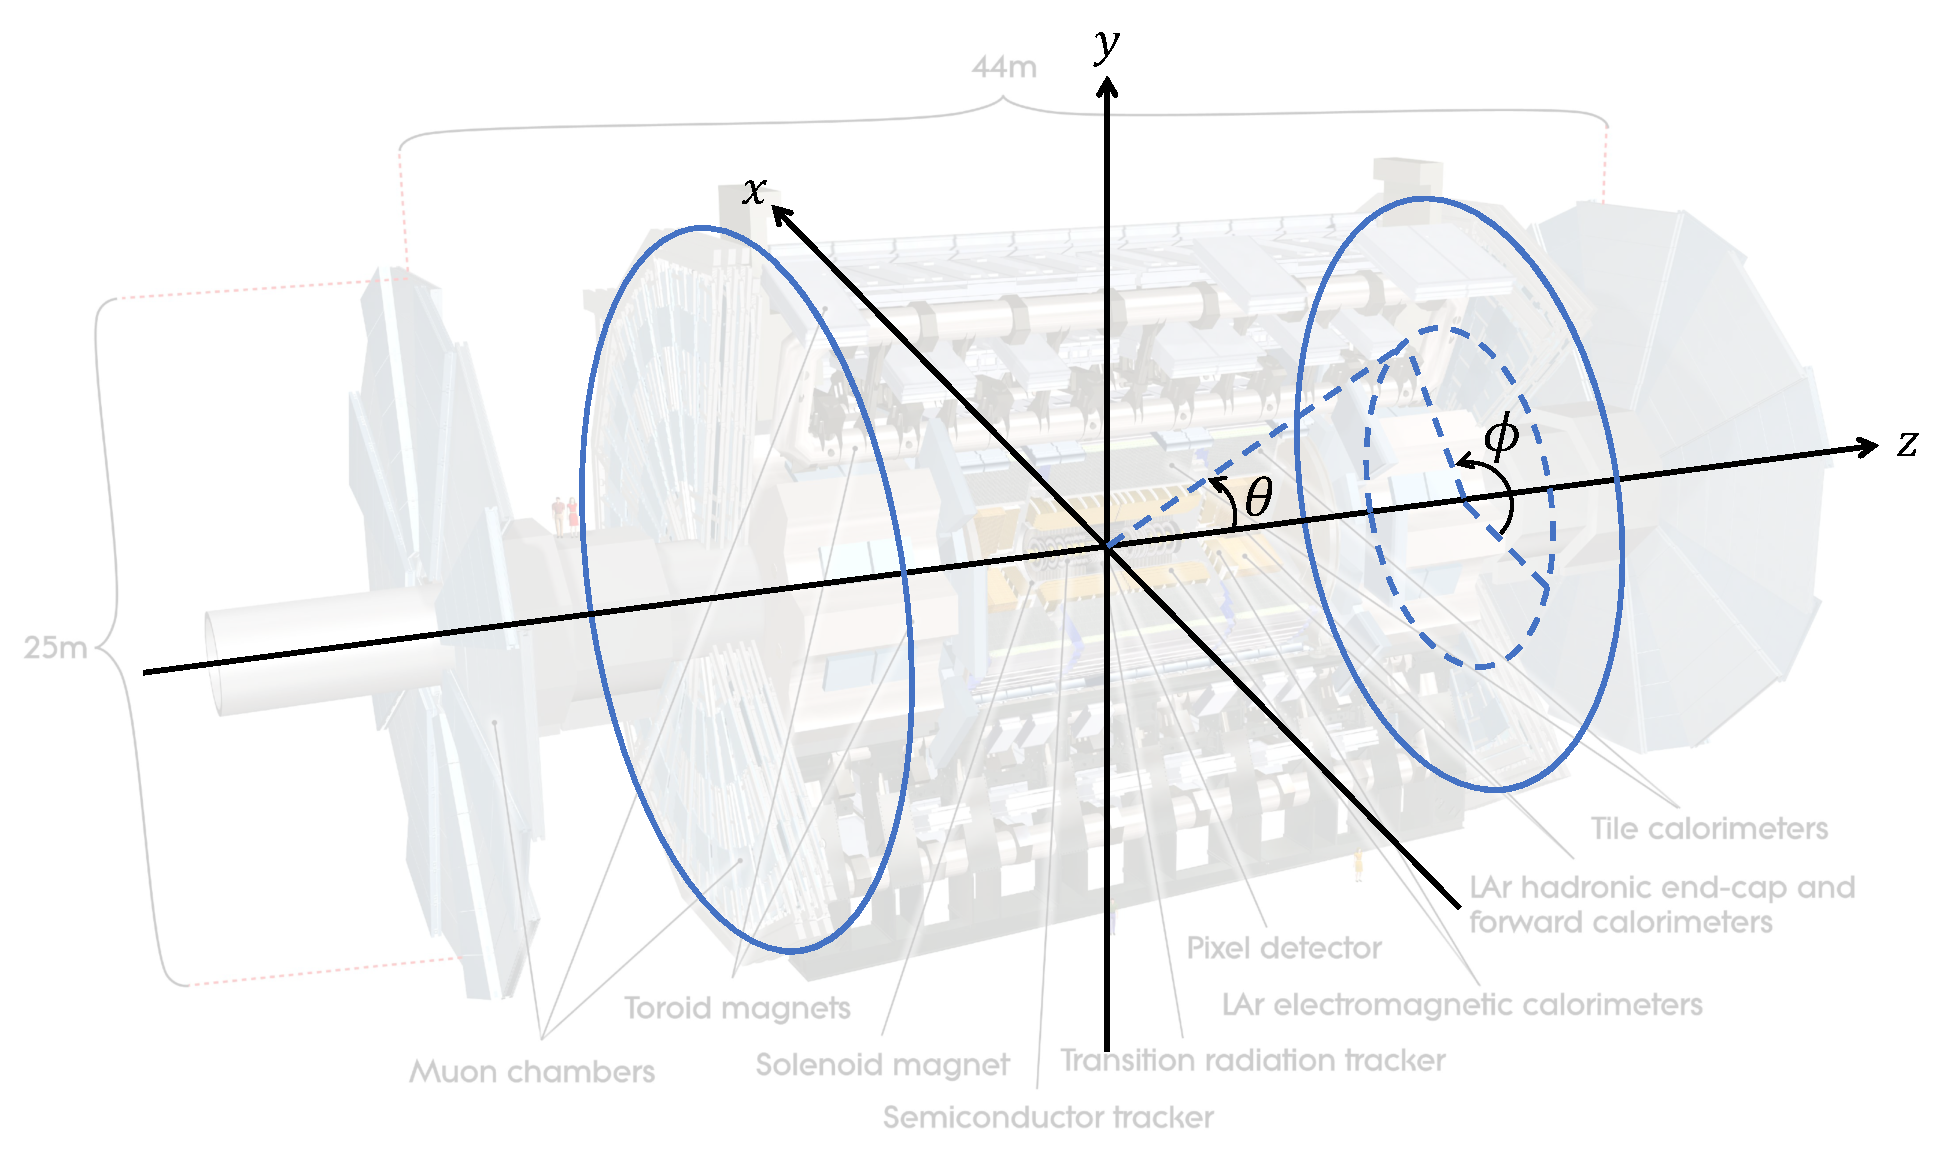
\includegraphics[clip, width=14cm]{fig/2/atlas_coordinate_fix.pdf}
  \caption{ATLAS検出器における座標系}
  \label{fig:a}
\end{figure}

\subsection{マグネットシステム}
ATLAS 実験では、荷電粒子の運動量測定のために超伝導磁石を用いている。超伝導磁石は 2 種類あり、1 つは衝突点付近で発生した荷電粒子の運動量測定のために用いられるソレノイド磁石であり、もう 1 つはミューオンの運動量測定のために用いられるトロイド磁石である。トロイド磁石はバレル部とエンドキャップ部に分けられ、それぞれ$\phi$ 方向に等間隔で 8 つずつ配置されている。ただし、バレル部とエンドキャップ部での磁場の干渉を考慮して、エンドキャップ部のトロイド磁石はバレル部に対して 22.5 度回転した状態で配置されている。

\subsection{内部飛跡検出器}
内部飛跡検出器は衝突点で発生した荷電粒子の飛跡を測定する。その際、荷電粒子の飛跡はソレノイド磁石によって曲げられる。この飛跡は荷電粒子の運動量の算出に用いられる。
内部飛跡検出器は内側から Insertable B-Layer (IBL)、ピクセル検出器、Semiconductor Tracker (SCT)、Transition Radiation Tracker (TRT) で構成されている。


\begin{figure}
    \centering
    \begin{minipage}[b]{0.4\linewidth}
        \centering
        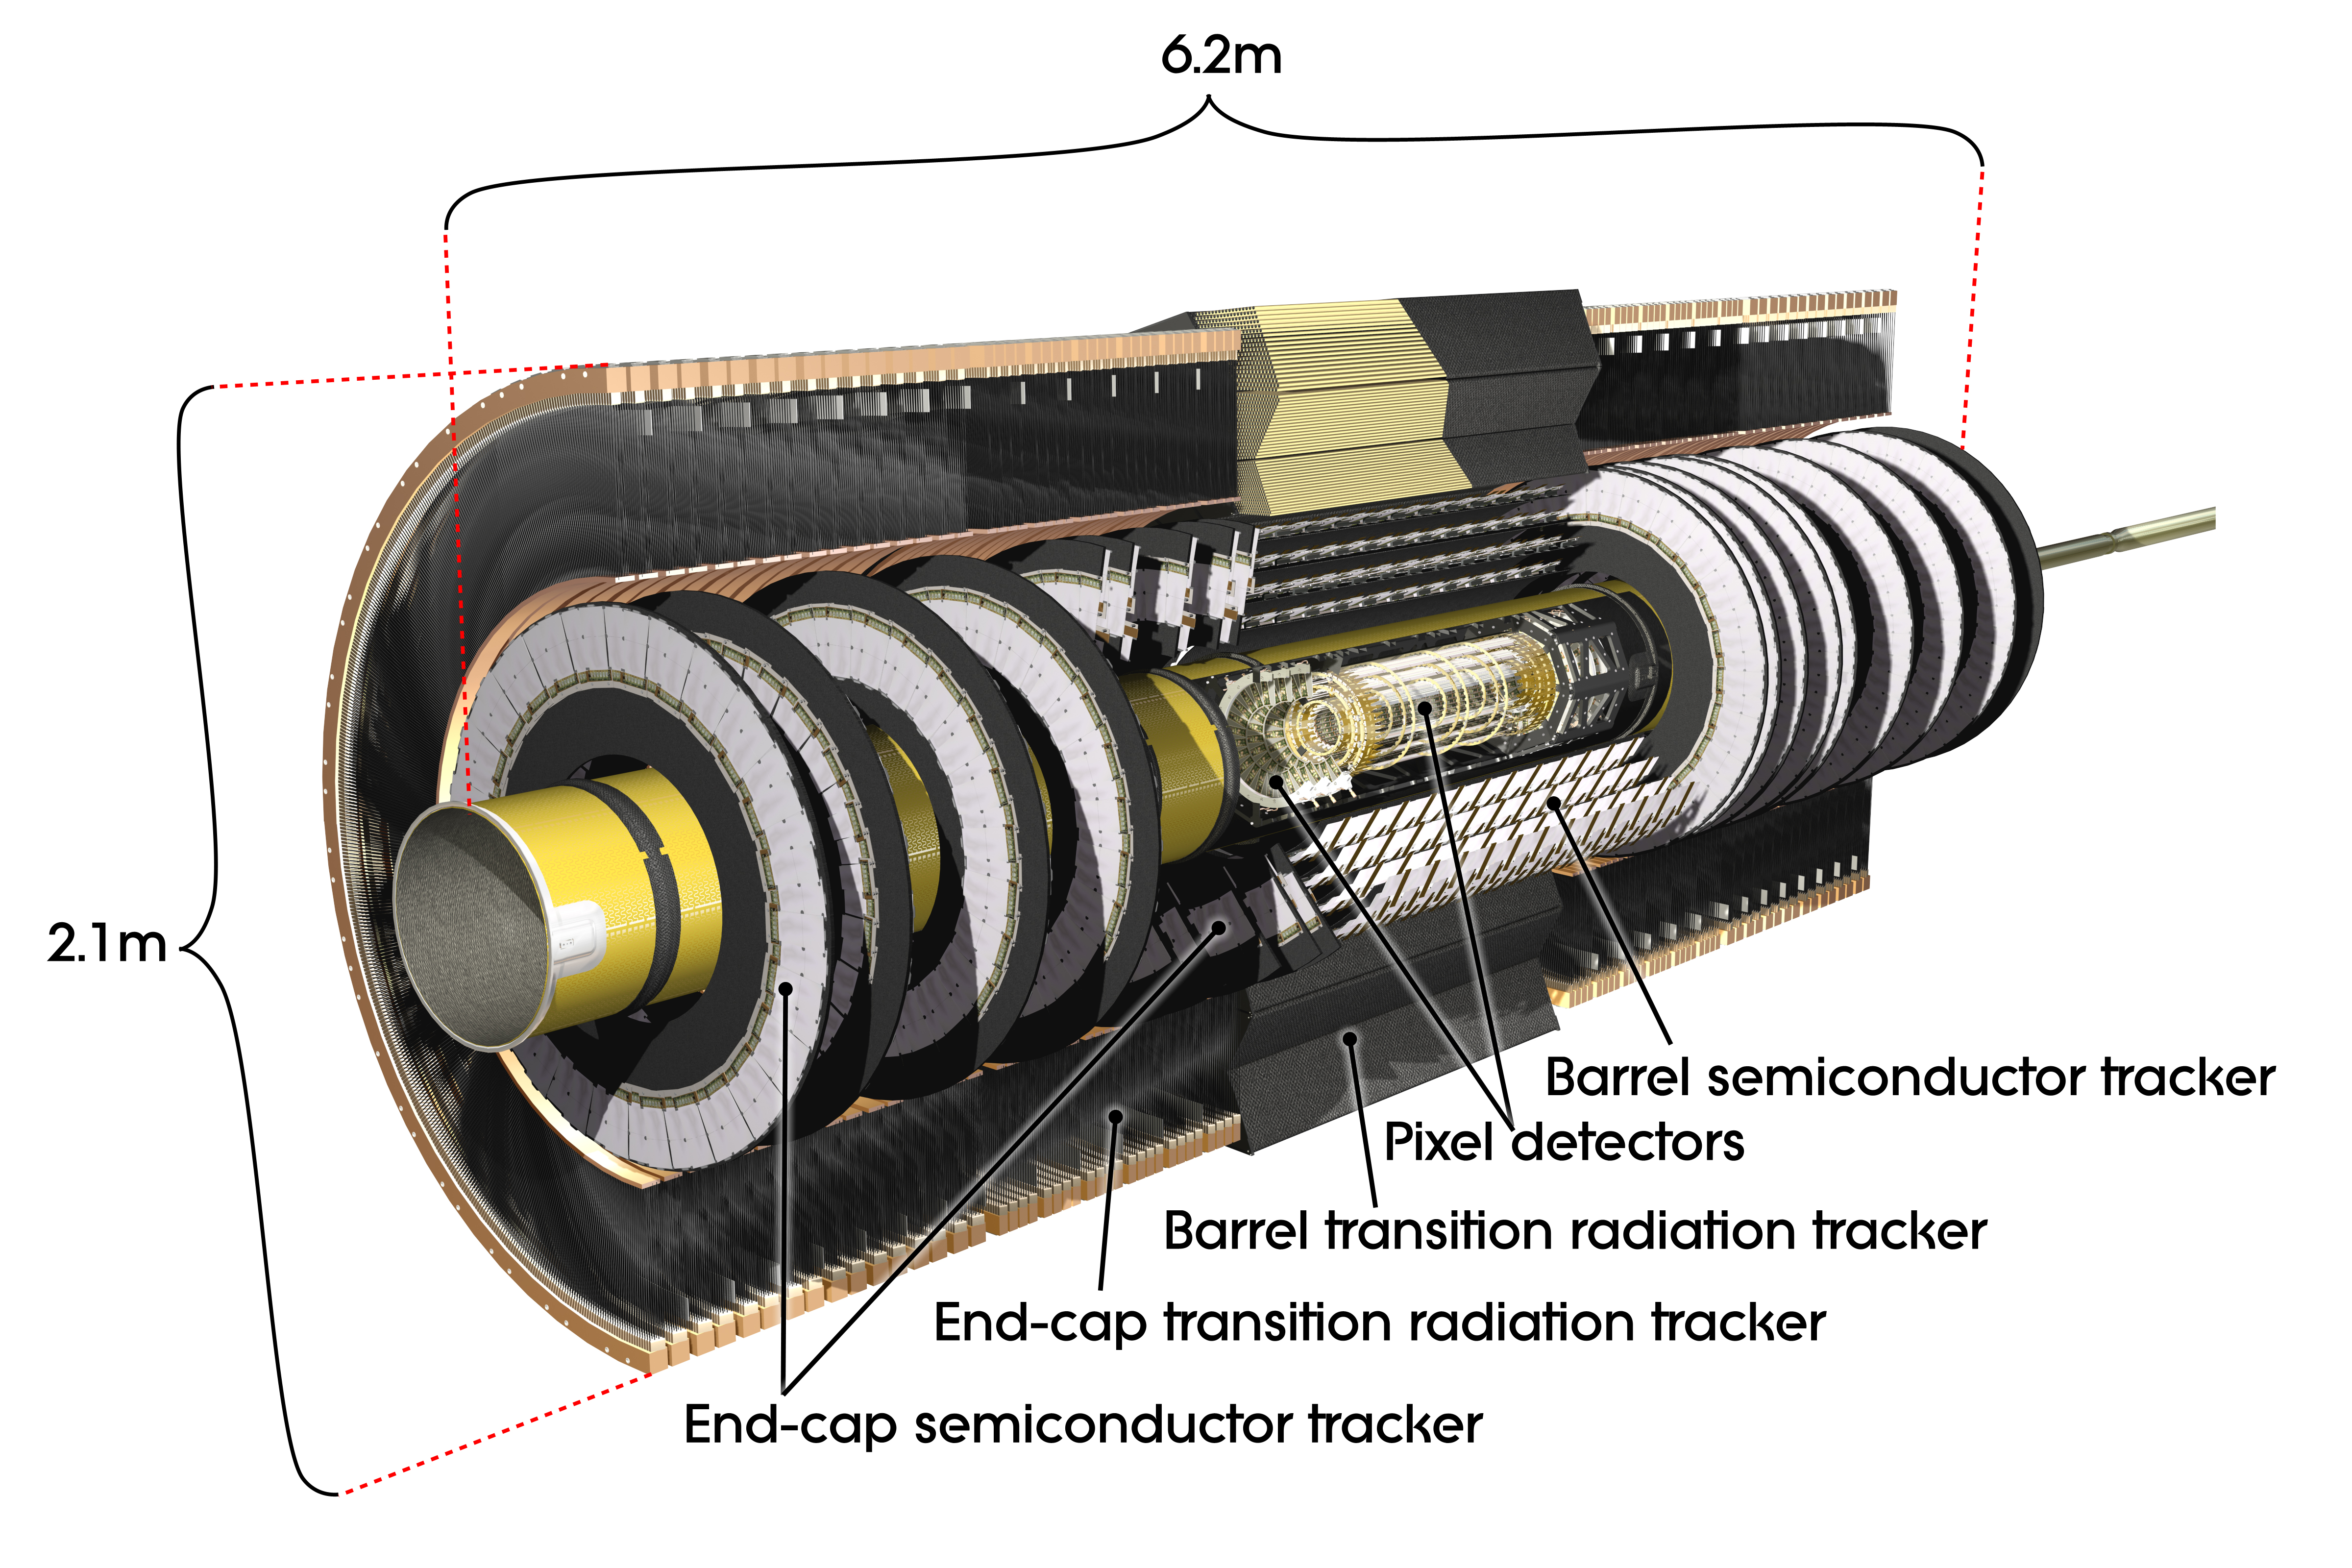
\includegraphics[clip, width=7cm]{fig/2/inner_detectoer1.jpg}
        \vspace{10pt}
        \subcaption{内部飛跡検出器の概略図}
        \label{fig:内部飛跡検出器の概略図1}
    \end{minipage}
    \hfill
    \begin{minipage}[b]{0.5\linewidth}
        \centering
        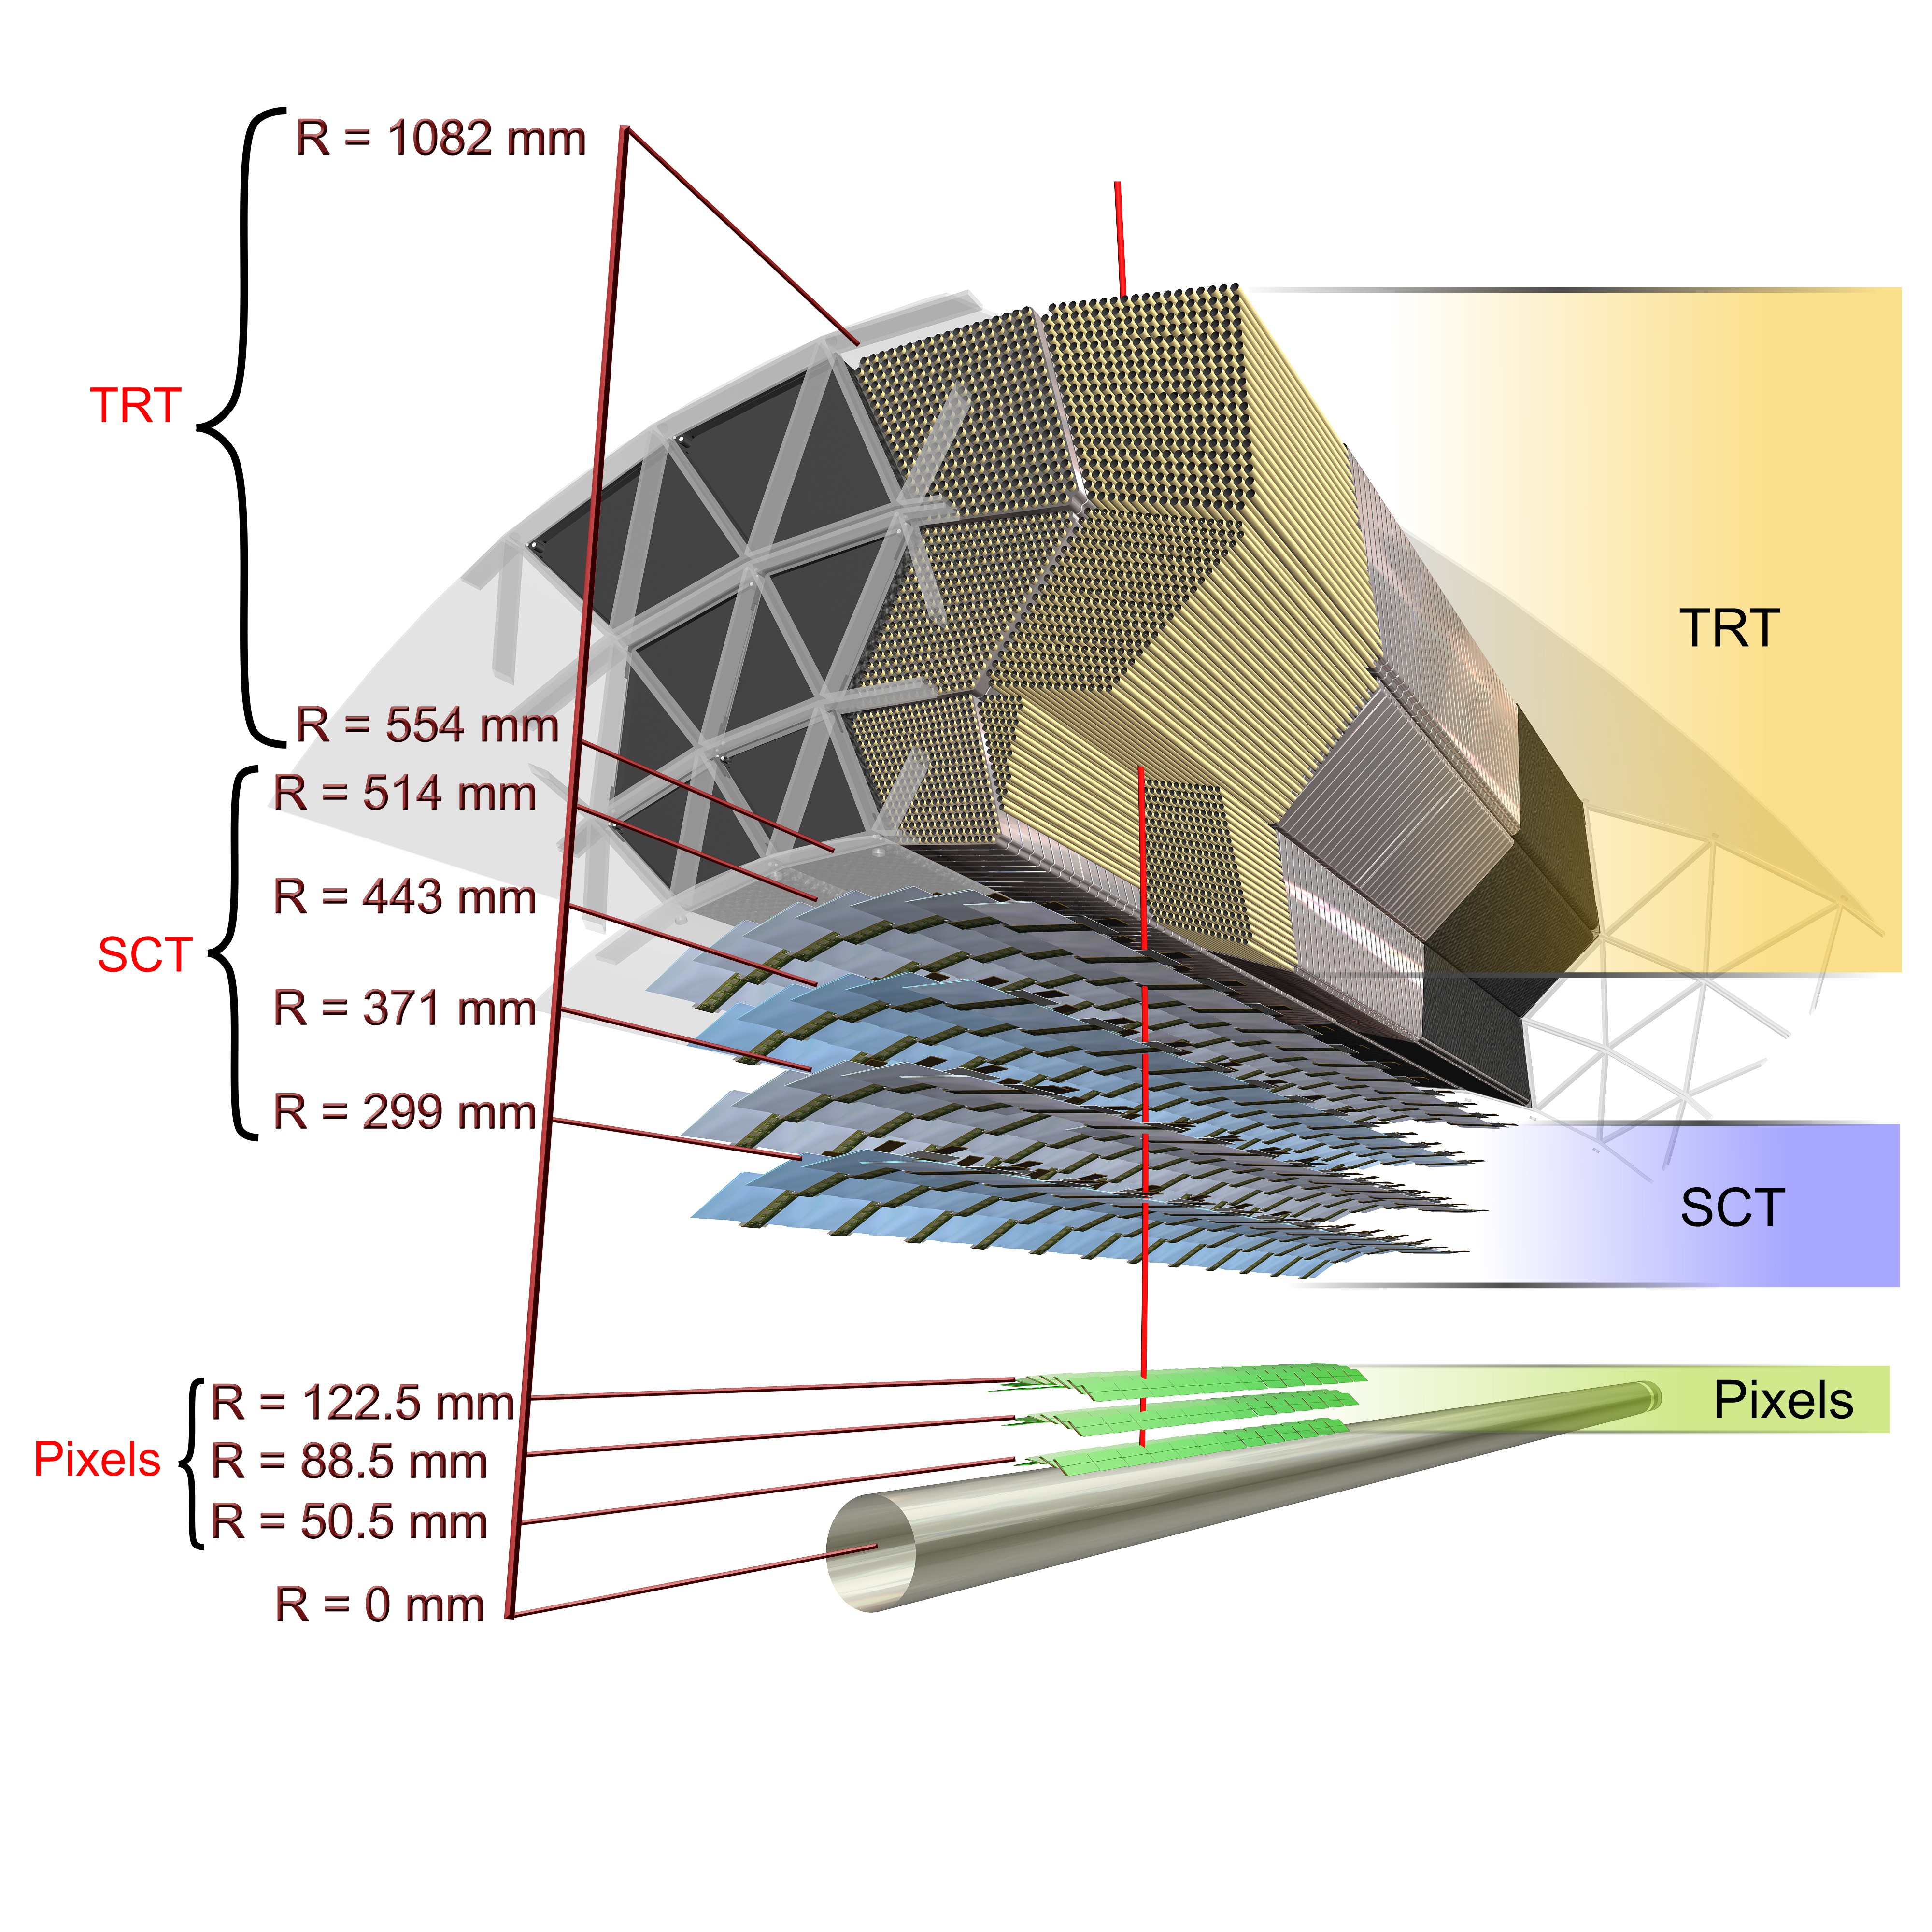
\includegraphics[clip, width=6cm]{fig/2/inner_detector2.jpg}
        \vspace{10pt}
        \subcaption{内部飛跡検出器の概略図}
        \label{fig:内部飛跡検出器の概略図2}
    \end{minipage}
    \caption{内部飛跡検出器}
    \label{fig:内部飛跡検出器}
\end{figure}



\subsection{カロリメータ}
カロリメータは、内部飛跡検出器の外側に設置されており、LHCでの陽子衝突で生成された粒子のエネルギー及び位置を測定する役割を担っている。
ATLAS検出器に設置されているカロリメータは、吸収層と検出層からなるサンプリングカロリメータであり、高密度物質の吸収層で粒子シャワーを起こし、検出層で電気信号に変えることで粒子の同定を行っている。
ATLASのカロリメータは、電磁カロリメータとハドロンカロリメータの2種類設置されている。

\subsubsection{・電磁カロリメータ}
電磁カロリーメーターは、$|\eta|<1.5$をカバーするバレルカロリメータと、$1.4<|\eta|<3.4$をカバーするエンドキャプカロリメータに分かれている。
バレル部とエンドキャプ部ともに、吸収層の鉛と検出層の液体アルゴンで構成されたカロリメータであり、電磁相互作用を起こす光子や電子のエネルギーと位置を測定する役割を担っている。

\subsubsection{・ハドロンカロリメータ}
ハドロンカロリメータは電磁カロリメータの外側に設置されており、タイルカロリーメータ、エンドキャップカロリーメータ、フォワードカロリーメータの3つに分類され、それぞれ異なる$|\eta=$範囲をカバーする。バレル部では、鉛と

\subsection{ミューオンスペクトロメータ}
\label{section2-2-4}

\subsubsection{・Resisitive Plate Chamber (RPC)}
\subsubsection{・New Small Wheel (NSW)}
\subsubsection{・Thin Gap Chambers (TGC)}
TGC は磁場領域より内側に EI (Endcap Inner) と呼ばれるステーション、磁場領域より外側に M1、M2、M3 (Middle 1,2,3) と呼ばれる 3 つのサブステーションが配置されている。磁場領域より外側にある M1 ステーションは TGC Triplet で構成されており、M2、M3 ステーションは TGC Doublet で構成されている。
M1、M2、M3 のヒット情報をトリガー判定に使用し、M3 はミューオントリガーの位置情報を決定するための基準として用いられているため、Pivot plane と呼ばれている。
磁場領域より内側にある EI ステーションは TGC Doublet で構成されており、これは EI チェンバーはトロイド磁石と干渉しないように配置されているため、図  のように一部の φ 領域のみをカバーしている。。TGC-EI のヒット情報を TGC-BW の飛跡情報とコインシデンスをとるために用いる。

\subsubsection{・Monitored Drift Tube (MDT)}
\subsubsection{・small-strip TGC (sTGC)}
\subsubsection{・Micromegas (MM)}










\chapter{初段ミューオントリガーシステム}\label{chapter3}
ATLAS実験における初段ミューオントリガーは、RPCを用いるバレル部とTGCを用いるエンドキャップ部に分かれている。
本章では、Run-3におけるエンドキャプ部の初段ミューオントリガーシステムについて述べる。

\section{エンドキャプ部初段ミューオントリガー}

\subsection{トリガーアルゴリズムの概要}\label{section:CW}

\subsubsection{ミューオンの横方向運動量の判定}

\subsubsection{インナーコインシデンス}\label{innnercoin}

\subsubsection{トリガー判定に用いられる位置情報}

%\newpage
\subsection{初段ミューオントリガーにおけるエレクトロニクス}

\subsubsection{Amplifier Shaper Discriminatorボード}

\subsubsection{Patch-Panel ASIC}

\subsubsection{Slave Board ASIC}

\subsubsection{High PT ボード}

\subsubsection{New Sector Logic}

\section{従来のCWの作成及び最適化手法}\label{section:最適化}
\subsection{従来のCWの作成方法}

\subsection{CWの最適化手法}
\subsubsection{TGCの設置位置の測定}\label{ズレ}


\subsubsection{Run-2における最適化手法}

\section{本研究の目的}
\chapter{機械学習を用いたCoincidence Windowの作成手法}\label{chapter4}
第\ref{chapter3}ではATLAS実験で実装されているトリガーシステムの概要について説明し、初段ミューオントリガーで使用されているCWの作成及びRun-2における最適化手法について述べ、効率的な最適化手法の開発が必要であることを示した。
本章では近年発展が著しい種々の機械学習についての概説を述べ、本研究の主題である機械学習を用いることで効率よくCWを作成及び最適化する手法について述べる。

\section{機械学習}\label{回帰分析}
機械学習は近年大きな注目を集めている技術であり、本研究の目的であるCWの作成作業の効率化に対する解決案として期待できる。
ここで機械学習とは、データからコンピュータが自動で特徴量やルールを学習し、学習した結果に基づいて新たなデータに対し分類や予測を行う分析手法の一つである。
代表的な分析手法として「クラス分類」と「回帰分析」がよく知られている。
クラス分類とは、分析したいデータが属するカテゴリーやクラス、種類が何なのかを判定する手法である。特に、予測するクラス数が 2 クラスの場合には 2 値分類と、2クラスより多い分類予測については多クラス分類と呼ばれる。図\ref{fig:class}にクラス分類の概要図を示す。高エネルギー物理学実験では、粒子の同定や探索の対象としている信号事象 (シグナル) とその背景事象 (バックグラウンド) の分離などに応用されている。
回帰の主な目的は、連続値などの値を学習データの傾向をもとに予測することである。過去の気温から明日の気温を予測することや企業における売り上げの予測などが回帰に当てはまる。回帰分析には、線形回帰、多項式回帰などが存在し、図\ref{fig:regre}に線形回帰の概要図を示す。線形回帰では,データから推定される線形予測関数を用いて傾向をモデル化する。高エネルギー物理学実験では、粒子の衝突で得られたデータを説明変数とし、粒子のエネルギー測定の補正を行う解析などに応用されている。

\begin{figure}[tb]
  \centering
    \begin{minipage}[b]{0.4\linewidth}
        \centering
        \includegraphics[clip, width=7cm]{fig/4/regression.png}
        \vspace{10pt}
        \subcaption{}
        \label{fig:regre}
    \end{minipage}
    \hfill
    \begin{minipage}[b]{0.4\linewidth}
        \centering
        \includegraphics[clip, width=7cm]{fig/4/classification.png}
        \vspace{10pt}
        \subcaption{}
        \label{fig:class}
    \end{minipage}
  \caption{機械学習の代表的な分析手法。(a):回帰分析、(b):クラス分類の概要図}
  \label{fig:fit_def}
\end{figure}

機械学習のトレーニング手法は、正解の値(教師データ)を与えた状態で傾向を学習させる「教師あり学習」と教師データを用いずに学習を行う「教師なし学習」の2つに大きく分けられる。
本研究では教師あり学習によって機械学習モデルのトレーニングを行う。
%教師あり学習は正解の値を与えた状態で傾向を学習させる方法である。
%教師あり学習は、「学習」と「予測」といった 2 つのプロセスによって成り立っており、、正解のデータを用いてルールやパターンの学習を行った後、新しいデータに対して、これまでに学習したデータを用いて予測を行う。
%一方で教師なし学習は、正解の値を教えずに学習させる方法である。大量のデータを学習させることでデータの特徴やパターンなどを覚えるが、それが正解か否かを判断することを学ぶのが教師なし学習の特徴である。
%また強化学習では、出力される結果に点数をつけて、最も多くの点数を得るための行動を学習させる。教師なし学習と同じように正解の値を学習させないが、教師なし学習との違いは、機械が報酬を得るために最適な行動を自ら考え実行する点である。

\subsection{ニューラルネットワーク}
機械学習には多くの種類があるが、その内の一つがニューラルネットワークを使った手法である。ニューラルネットワークとは、人間の脳内にある神経細胞(ニューロン)とそのつながり、つまり神経回路網を人工ニューロン(パーセプトロン)という数式的なモデルで表現したものである。個々のパーセプトロンは単純な仕組みであるが、多数組み合わせる事で複雑な関数近似を行う事ができるのが、ニューラルネットワークの大きな特徴である。

図~\ref{fig:perce}に示すように、パーセプトロンは入力と出力の2層で構成され、 n 個の信号$x_i$に対し重み$w_i$を作用させバイアス b とともに入力し、1個の信号$y$を出力する関数 $f(x_i; w_i)$ を持ったモデルである。式~\eqref{equ:acctivation}で表すことができる。この $f(x_i; w_i)$ の事を「活性化関数」と呼び、活性化関数には、sigmoid 関数、tanh 関数、ReLU 関数~(Rectified Linear Unit)」、 softmax 関数などが良く使われている。 
\begin{equation}
    %y = f(\Vec{w}・\Vec{x} + b)
    y = f(x_i; w_i) = \sum^{n-1}_{i=1}(w_i・x_i) + b
    %f \begin{pmatrix}  \\ 2 & 3 \end{pmatrix}
    \label{equ:acctivation}
\end{equation}
\begin{figure}[tb]
  \centering
  \includegraphics[clip, width=13cm]{fig/4/parceptron.png}
  \caption{単一パーセプトロンの概念図。}
  \label{fig:perce}
\end{figure}
sigmoid 関数及びReLU 関数の概形を図\ref{fig:sigmoid},図\ref{fig:ReLU}に示す。sigmoid 関数はニューラルネットワークでよく用いられてきた関数であり、式\eqref{equ:sigmoid}のような関数で表される。ReLU 関数は式\eqref{equ:ReLU}のような関数で示される。
\begin{equation}
    y = \frac{1}{1+exp(-x)}
    %f \begin{pmatrix}  \\ 2 & 3 \end{pmatrix}
    \label{equ:sigmoid}
\end{equation}

\begin{equation}
    y = max(0,x)
    %f \begin{pmatrix}  \\ 2 & 3 \end{pmatrix}
    \label{equ:ReLU}
\end{equation}

\begin{figure}
    %\centering
    \begin{tabular}{cc}
    \begin{minipage}[b]{0.45\hsize}
        %\centering
        \includegraphics[clip, width=7cm]{fig/4/sigmoid_2.pdf}
        %\vspace{5pt}
        \subcaption{}
        \label{fig:sigmoid}
    \end{minipage}&
    %\hfill
    \begin{minipage}[b]{0.45\hsize}
        %\centering
        \includegraphics[clip, width=7cm]{fig/4/ReLU_2.pdf}
        %\vspace{5pt}
        \subcaption{}
        \label{fig:ReLU}
    \end{minipage}
    \end{tabular}
    \caption{機械学習で用いられる活性化関数の例。(a): sigmoid 関数、(b): ReLU 関数。}
    \label{fig:acctivation}
\end{figure}
\subsection{多層パーセプトロン}
単一のパーセプトロンでの分析は単純なものであれば問題ないが、複雑な事象を扱うことは難しい。そこで、このパーセプトロンを複数組み合わせることにより多層化することで、複雑な表現を可能とした多層パーセプトロン (MLP : Multilayer perceptron) が考案された。
単一のパーセプトロンは入力と出力のみであったのに対し、図\ref{fig:MLP}に示すように、MLP は隠れ層と呼ばれる層が複数追加されたネットワーク構造を持ち、各層間は全結合しているような構造になっている。この様な構造を持つニューラルネットワークの事を「全結合型ニューラルネットワーク」と呼ぶ。出力層においてよく使われる主な活性化関数としては、2種類の分類問題に対しては sigmoid 関数、多クラスの分類問題に対しては softmax 関数、回帰問題に対しては linear 関数などが用いられる。
\begin{figure}[tb]
  \centering
  \includegraphics[clip, width=10cm]{fig/4/MLP_re.png}
  \caption{MLP の概形。パーセプトロンを複数組み合われており、ある層のパーセプトロンからの出力は全結合されて次の層の各パーセプトロンに入力される。}
  \label{fig:MLP}
\end{figure}

出力された予測値は損失関数を用いて評価が行われる。これは、入力値 $x_n$ に対してとある重み $w$ を設定して予測値 $y$ を導出し、その予測値 $y$ に対し目標値 $t$ との誤差 $L$ が最小になるようにそれぞれの重みやバイアスなどのパラメータの値を少しだけ増減させ調整を行う方法である。この調整を繰り返すことによって予測の精度を向上させていく。図\ref{fig:lossfunction}にパラメータの更新の流れを示す。
この調整の際に使用される誤差を計算する関数は「損失関数」と呼ばれ、特に式~\eqref{equ:MSE}に示すような関数で表される平均二乗誤差~(MSE : Mean Squared Error)が多く用いられる。他には、平均絶対誤差~(MAE : Mean Absolute Error)や平均二乗誤差の平方根~(RMSE : Root Mean Squared Error)などが用いられる。
また、学習の中で重みやバイアスの値の更新を行う回数をepochと呼び、一度の重み更新で変更する重みの大きさを調節する学習率~(Learning rate)などと合わせてハイパーパラメータとして設定する。

\begin{equation}
    L = \frac{1}{n}\sum^{n}_{i=1}(y_i-t_i)^2
    %f \begin{pmatrix}  \\ 2 & 3 \end{pmatrix}
    \label{equ:MSE}
\end{equation}

\begin{figure}[tb]
  \centering
  \includegraphics[clip, width=10cm]{fig/4/lossfunc_laerning.png}
  \caption{損失関数 $L$ の最小化の流れ。ある重み $w_i$ の時の勾配 $\frac{\partial L}{\partial w}$ を計算し、この勾配が小さくなるように重みを更新することを繰り返す。この際、更新量を調整するために学習率 $\eta$ を設定する。バイアス $b$ に対しても同様に最小化を行う。}
  \label{fig:lossfunction}
\end{figure}


\section{機械学習を用いた CW 作成手法}
本節では機械学習の学習方法及びCWを作成する手法について述べる。
従来の作成手法では、シミュレーションデータを用いて$p_T$閾値を決定しCWを作成する。その後、実際のデータを使用して磁場の影響や検出器のズレに最適化させるといった方法を行っていた。一方、本研究で開発する作成手法では実際のデータを学習に利用した機械学習を用いてミューオンの$p_T$の予測を行い、予測した$p_T$を使用してCWを作成する。また、本研究で作成するCWは実際の測定で用いるトリガー用のCWの他にシミュレーションで用いるトリガー用のCWもシミュレーションデータを用いて同様の手法で作成する。

初めに、トレーニングに使用するシミュレーションデータおよび実際のデータを学習に適した形式に変更する。次に図~\ref{fig:MLP_over}に示すように、TGCにおけるミューオンのヒット位置の情報を表すトリガーセクターの番号とRoIの番号、ミューオンの飛跡の曲がり具合を表す($\Delta R$, $\Delta \phi$)の4変数から$p_T$の値を出力するMLPをトレーニングする。この時、機械学習の分析手法として回帰分析を行うため、出力される値は連続値となる。出力された$p_T$の値を15段階の閾値に変換するために、任意の値で$p_T$を区切っり、トリガー効率を求めTurn-on curve にフィッティングを行うことで15段階の$p_T$閾値に対応したCWを作成する。

\begin{figure}[tb]
  \centering
  \includegraphics[clip, width=15cm]{fig/4/MLPoverview.png}
  \caption{機械学習を用いた CW 作成の流れ。$\Delta R$, $\Delta \phi$ RoI, トリガーセクターの情報の 4 変数を入力値、横方向運動量$p_T$を出力値とした機械学習を用いる。出力された$p_T$は連続値であり、これを15段階の$p_T$閾値に変換することで CW を作成する。}
  \label{fig:MLP_over}
\end{figure}

\subsection{入力データに対する事前処理}\label{事前処理}
本節では学習に用いるシミュレーションデータおよび実際のデータに対して処理を行い、本研究の機械学習に適した形式に変換する方法について述べる。

本研究ではトレーニングのために、シミュレーションデータ及び実際の測定データを使用する。
シミュレーション用のCWを作成するための機械学習のトレーニングには、1回のイベントに対してミューオンが1個存在するシングルミューオンのシミュレーションサンプルを使用する。オフライン再構成されたミューオンに対して、TGCのM3におけるヒット情報が存在することを要求する。そして、TGC M3におけるヒット情報からヒット位置の情報(トリガーセクターの番号、RoIの番号)と飛跡の情報($\Delta $、d$\phi$)を取得する。
また、実際の測定に使用するCWを作成するための機械学習のトレーニングには、2018年Run-2で収集されたデータを用いる。使用するイベントにはHLTのシングルミューオントリガーである「HLT$\_$mu26$\_$ivarmeduium」を要求する。シミュレーションデータと同様に、イベントの中でもTGC M3おけるヒット情報が存在するオフライン再構成されたミューオンをすべて使用し、TGC M3におけるヒット位置の情報(トリガーセクターの番号、RoIの番号)と飛跡の情報($\Delta$ R、d$\phi$)を取得する。

%\begin{figure}[thb]
%  \centering
%  \rule{8cm}{6cm}
%  %\includegraphics[clip, width=14cm]{}
%  \caption{深層学習モデルのトレーニングに用いたシングルミューオンサンプルの $p_T$ 分布。}
%  \label{fig:mu_pt_forMC}
%\end{figure}

%\begin{figure}[thb]
%  \centering
%  \rule{8cm}{6cm}
%  %\includegraphics[clip, width=14cm]{}
%  \caption{深層学習モデルのトレーニングに用いたミューオンの $p_T$ 分布。}
%  \label{fig:mu_pt_forData}
%\end{figure}

\subsubsection{TGCの位置情報におけるナンバリングの変換}
学習には、TGCのヒット位置の情報としてトリガーセクターの番号とRoIの番号を使用する。
\ref{fig:TGCnumbering}に示すようにRoIはトリガーセクターごとに設定された番号が与えられており、あるトリガーセクターの一番端の列のRoIの番号は隣接するトリガーセクターのRoIの番号と関連性がない。
しかし、隣り合った場所に位置するRoIは似通った磁場構造を持っているため、トレーニングするにあたって、隣り合ったRoIの情報に関連性を持たせたい。

\begin{figure}[tb]
  \centering
  \includegraphics[clip, width=12cm]{fig/4/TGC_numbering.pdf}
  \caption{TGCにおけるトリガーセクターとRoIのナンバリングの概要。}
  \label{fig:TGCnumbering}
\end{figure}

本研究では、TGCにおけるヒット位置を表すトリガーセクターの番号とRoIの番号を、新たに隣り合ったRoIの番号が連続するようなナンバリングに変換する。
図~\ref{fig:newnumbering}に新たなナンバリングの概要を示す。Eta$\_$IndexはRoIを$\eta$方向に0から37の番号に、Phi$\_$IndexはRoIを$\phi$方向に0から191の番号に読み替えている。
\begin{figure}[tb]
  \centering
  \includegraphics[clip, width=14cm]{fig/4/new_numbering.pdf}
  \caption{新たなナンバリングの概要。マスの中で数字はRoIの番号を表しており、奇数の番号のトリガーセクターでは読み出し回路の関係からRoIのナンバリング順が反転している。TGCにおけるヒット位置の情報(Sector番号、RoI番号)を新たに(Eta$\_$Index, Phi$\_$Index)で指定する。}
  \label{fig:newnumbering}
\end{figure}

\subsubsection{磁場構造を考慮した学習領域の分割}
\ref{magnetic_filed}節で述べたように、トロイド磁石が8回転対象に設置されていることにより TGC-BW における磁場構造は図\ref{fig:Mag}に示すように一様ではない。そのため、本研究ではTGC-BWの全領域を一つの機械学習でトレーニングさせるのではなく、図\ref{fig:Mag}で色付けされた領域が示すように、入力データとして使用する領域を分割して複数の機械学習をトレーニングする。
本研究では、磁場構造に考慮するためにTGC のエンドキャプ部を $\phi$ 方向に 48 分割、$\eta$ 方向に 9 分割、フォワード部を $\phi$ 方向に 24 分割、$\eta$ 方向に 4 分割にし、それぞれの領域に対して機械学習のトレーニングを行う。
\begin{figure}[tb]
  \centering
  \includegraphics[clip, width=9cm]{fig/4/c1_withMag.pdf}
  \caption{磁場構造を考慮するための学習領域の分け方。赤色の領域に対するトレーニングを行う際には緑色で囲まれたの領域のデータを使用する。}
  \label{fig:Mag}
\end{figure}

\subsubsection{ミューオン情報の選別}
次に各RoIにおけるヒットマップを作成し学習に使用するミューオンの選別を行う。作成したヒットマップには孤立しているマスが存在する。
これは偶発的にミューオンがヒットしたことや多重散乱の影響によるもので、このままトレーニングに用いると本来$p_T$を判定する必要のないマスまで学習してしまい、トリガーレートの増加に繋がってしまう。
そのため、以下に説明する手順に沿ってヒットマップを用いたミューオンの選別行う。
図~\ref{fig:hitmapcleaner}にヒットマップクリーナを作用させた場合の例を示す。
\begin{enumerate}
   \item エントリー数が 3 以下のマスは削除する。これは、偶発的にミューオンがヒットしたマスを削除することを目的とする。
   \item あるマスに隣接する周囲の8マスのうち、ミューオンがヒットしたマスが2マス以下であるとき、削除する。これは、孤立したミューオンのヒットを削除することを目的としている。
\end{enumerate}


\begin{figure}[tb]
  \centering
  \includegraphics[clip, width=14cm]{fig/4/cleaner.png}
  \caption{ヒットマップクリーナーをかけた前後のミューオンヒットマップの例}
  \label{fig:hitmapcleaner}
\end{figure}


\subsection{機械学習モデルの設計方法とトレーニング}
本節では飛跡の曲がり具合と TGC$\_$BW のヒット情報からミューオンの横方向運動量 $p_T$ を出力させる機械学習モデルの設計について述べる。

\subsubsection{機械学習モデルの設計}
本研究において、機械学習モデルの構築にはGoogle社によって開発された機械学習に用いるためのオープンソースのフレームワークであるTensorFlow~\cite{article:TensorFlow}とニューラルネットワークライブラリであるKeras~\cite{article:keras}を用いた。

本研究で使用する機械学習モデルは、4つの入力変数を持つ入力層、5つの隠れ層、$p_T$ の値を出力する1つの出力層となるような、回帰分析を行う全結合型MLPモデルを構築する。
図~\ref{fig:MLP_overview}に機械学習モデルの概要図を示す。
MLPの各隠れ層は以下の表\ref{table:hibben}に示す要素から構成される。
\begin{enumerate}\label{table:hibben}
   \item Dence layer:前の層からのすべての出力の線形結合を入力としたパーセプトロンの層。1 つの層に存在するパーセプトロンの数をノード数と呼ぶ。
   \item Batch normalization layer:入力に対し正規化を行う層。
   \item Dropout unit:学習中にランダムに選ばれたノードの一定割合をゼロにする操作。過学習の抑制のために用いられ、ドロップアウトする割合はハイパーパラメータとして設定する。
   \item Activation unit:活性化関数を設定する層。
   %\caption{隠れ層を構成する要素。}
\end{enumerate}
出力層には ReLU 関数を活性化関数として使用する。これは、目的とする出力の $p_T$ の値が必ず正の値を取るためである。
誤差逆伝搬法にはRMSpropを用いて勾配降下法を行っている。

\subsubsection{ハイパーパラメータ}
隠れ層の数、ノード数、ドロップアウト率、損失関数、学習率の 5 個のハイパーパラメータを表\ref{table:hyper}のように変化させることで評価を行い最適なモデルを選択した。評価にはPreferred Networks社が開発したハイパーパラメータの最適化を自動で行うフレームワークである Optuna \cite{article:optuna}を使用した。
\begin{enumerate}\label{table:hyper}
   \item 隠れ層の数:3層 から 6層
   \item ノード数:128, 256, 512, 1024
   \item ドロップアウト率:0.01, 0.02, 0.03, 0.04, 0.05
   \item 活性化関数:Sigmoid 関数、ReLU 関数
   \item 学習率:0.01, 0.001, 0.0001
   %\caption{変化させるハイパーパラメータの一覧。}
\end{enumerate}
評価を行った結果、いくつかの組み合わせで同等の性能が得られることがわかった。これらのうち、学習可能なパラメータの数が最も少ないネットワークが選ばれた。パラメータとその値は、ドロップアウト率 0.05、活性化関数 ReLU、学習率 0.001, そして、5つの隠れ層と [256, 256, 256, 256, 256] のノード数を選択する。

\begin{figure}[tb]
  \centering
  %\rule{8cm}{6cm}
  \includegraphics[clip, width=12cm]{fig/4/MLP_2.pdf}
  \caption{機械学習モデルの概要図。4つの入力、各層に256個のノードを持つ5つの隠れ層、$p_{T}^{\rm{offline}}$を出力とする全結合型MLPを構築する。活性化関数はReLU、ドロップアウト率は0.05とする。}
  \label{fig:MLP_overview}
\end{figure}


\subsubsection{トレーニング}
機械学習モデルのトレーニングには、\ref{事前処理}節で述べた方法を用いて実際のデータ及びシミュレーションデータに対して事前処理を行ったデータを入力データとする。教師データとしてはそれぞれのデータでオフライン再構成されたミューオンの$p_T$を利用する。
トレーニングデータの総数は、シミュレーションデータが500万イベント、2018年Run-2データが約****万イベントである。

図~\ref{fig:epoch}に機械学習モデルをトレーニングした際のepochに対する出力と教師データの平均二乗誤差の推移を示す。全てのモデルにおいて validation データの平均二乗誤差は十分に収束している事が見て取れる。

\begin{figure}[tb]
  \centering
  %\rule{8cm}{6cm}
  \includegraphics[clip, width=7cm]{fig/4/epoch2.png}
  \caption{機械学習モデルをトレーニングした際の epoch に対する平均二乗誤差の推移。}
  \label{fig:epoch}
\end{figure}


\newpage
\subsubsection{機械学習モデルの性能評価}
まず、シミュレーションデータをもとにトレーニングを行った機械学習モデルについての評価を行う。
新たに500万イベントのシングルミューオンのシミュレーションデータ作成し評価に用いて、MLPで予測した$p_{T}^{pred}$とオフライン再構成された正解値 $p_{T}^true$ の比較を行った結果を図~\ref{fig:zannsa_25_MC}に示す。
また、ある$p_T^{True}$に対して、$p_T^{Pred}$の分布をガウシアンフィットした場合の$\mu$の分布を図~\ref{fig:Gausmu_MC}に示す。$p_T^{True}$に対して機械学習の予測値はほぼ線形である事が見て取れる。

\begin{figure}[tb]
  \centering
  %\rule{8cm}{6cm}
  \includegraphics[clip, width=11cm]{fig/4/zansa_25_MC.pdf}
  \caption{シミュレーションデータを用いてトレーニングを行ったMLPの$p_{T}^{True}$に対する$p_{T}^{Pred}$の分布。評価にはシングルミューオンのシミュレーションデータを用いた。}
  \label{fig:zannsa_25_MC}
\end{figure}

\begin{figure}[tb]
  \centering
  %\rule{8cm}{6cm}
  \includegraphics[clip, width=11cm]{fig/4/tp_Gausmean_MC.pdf}
  \caption{ある$p_T^{True}$に対して、$p_T^{Pred}$の分布をガウシアンフィットした場合の$\mu$の分布。}
  \label{fig:Gausmu_MC}
\end{figure}

次に、実際のデータをトレーニングに使用した機械学習モデルの評価を行う。
2018年Run-2で収集したデータを用いて、MLP で予測した$p_{T}^{pred}$ と正解値 $p_{T}^true$ の残差分布の比較を行った結果を図~\ref{fig:zannsa_25_Data}に示す。また、ある$p_T^{True}$に対して、$p_T^{Pred}$の分布をガウシアンフィットした場合の$\mu$の分布を図~\ref{fig:Gausmu_Data}に示す。こちらも$p_T^{True}$に対して機械学習の予測値はほぼ線形である事が見て取れる。

\begin{figure}[htb]
  \centering
  %\rule{8cm}{6cm}
  \includegraphics[clip, width=11cm]{fig/4/zansa_25_DESDM.pdf}
  \caption{2018年Run-2のデータを用いてトレーニングを行ったMLPの$p_{T}^{True}$に対する$p_{T}^{Pred}$の分布。評価には2018年Run-2のデータを用いた。}
  \label{fig:zannsa_25_Data}
\end{figure}

\begin{figure}[htb]
  \centering
  %\rule{8cm}{6cm}
  \includegraphics[clip, width=11cm]{fig/4/tp_Gausmean_Data.pdf}
  \caption{ある$p_T^{True}$に対して、$p_T^{Pred}$の分布をガウシアンフィットした場合の$\mu$の分布。}
  \label{fig:Gausmu_Data}
\end{figure}






\subsection{出力データをPt閾値に変換}
\subsubsection{トリガー効率の算出}
全オフライン再構成されたミューオンの内、あるpT 閾値以上のトリガーが発行された割合$\epsilon$を式~\eqref{equ:Eff}と定義し、トリガー効率の算出を行った。
このとき得られるトリガー効率を $p_T$ の関数で表したプロットをTurn-on curveと呼ぶ。
\begin{equation}
    \epsilon = \frac{ある p_T 閾値以上のトリガーを発行したミューオンの数}{全オフライン再構成したミューオンの数}
 \label{equ:Eff}
\end{equation}


\subsubsection{フィッティング関数の定義}\label{section:fitting}
式~\eqref{equ:fitting}を用いて Turn-on curve にフィッティングを行うことでトリガー効率を定量的に評価する。
\begin{equation}
    f(p_T) = \frac{p_0}{exp(\frac{p_T-p_1}{p_2})+1}
 \label{equ:fitting}
\end{equation}
ここで、トリガーの性能を表す 3 つのパラメータ $p_0$, $p_1$, $p_2$ を以下のように定義する。Turn-on curveにフィッティングした様子を図~\ref{fig:fiting}に示す。
\begin{figure}[tb]
  \centering
  \includegraphics[clip, width=12cm]{fig/4/fitting_def.png}
  \caption{Turn-on curve に対するfittingの例。$p_0$ を Plateau efficiency、$p_1$ を Effective threshold、$p_2$ を Resolution と定義する。}
  \label{fig:fiting}
\end{figure}

\begin{enumerate}\label{table:fitting}
   \item $p_0$:Plateau efficiency\\
   Turn-on curve が横這いになった時のトリガー効率を表す。トリガー閾値以上の pT を持つミューオンに対するトリガー効率を表すため、その値が 1 に近い方が高性能である。
   \item $p_1$:Effective threshold\\
   トリガーの実効的な $p_T$ の閾値を表す。トリガー効率が Plateau efficiency の値の 50\% となる時の $p_T$ の値である。
   \item $p_2$:Resolution\\
   トリガーの運動量の分解能を表す。Turn-on curve の立ち上がりの鋭さに対応すしており、Resolution の値が大きくなると Turn-on curve の立ち上がりが緩くなるため、fトリガーの運動量分解能が悪くなる。
\end{enumerate}

\subsubsection{15段階閾値への変換}
目的とする$p_T$の値はMLPから連続値として出力される。そのため、任意の値で$p_T$を区切り15段階の$p_T$閾値に変換を行う。
方法としては、任意の値で$p_T$を区切った時のトリガー効率を求め、Turn-on curveに対し式\eqref{equ:fitting}を用いてフィッティングを行う。フィッティング結果からEffective thresholdを求め、Effective thresholdが\ref{section:CW}節で述べたRun-3における15段階閾値となる任意の値を導出する。
本研究では出力された$p_T$を1GeVから30GeVまで0.1GeV刻みで区切り、それぞれのTurn-on curveに対してのフィッティング結果から15段階の$p_T$閾値に変換を行った。
図~\ref{fig:Effictive_thr_v1}に出力データを0.1GeV刻みで区切った時のEffective thresholdを示す。
\begin{figure}[tb]
  \centering
  \includegraphics[clip, width=12cm]{fig/4/Effictive_thr_v1.pdf}
  \caption{出力された$p_T$を0.1GeV刻みで区切った時のTurn-on curveにおけるEffective threshold。}
  \label{fig:Effictive_thr_v1}
\end{figure}
本研究では、フィッティング結果から表~\ref{Effective_number}のように15段階閾値に区切る値を決定した。
\begin{table}[thb]
\centering
    \caption{機械学習からの出力値におけるの15段階閾値。}
    \label{Effective_number}
    \begin{tabular}{|c|c|}
        \hline
        $p_t$ number & 出力された $p_T$ [GeV]\\
        \hline
        1 & 1.0\\
        \hline
        2 & 2.0\\
        \hline
        3 & 3.0\\
        \hline
        4 & 4.7\\
        \hline
        5 & 6.2\\
        \hline
        6 & 7.4\\
        \hline
        7 & 8.4\\
        \hline
        8 & 9.6\\
        \hline
        9 & 10.6\\
        \hline
        10 & 11.7\\
        \hline
        11 & 12.8\\
        \hline
        12 & 13.9\\
        \hline
        13 & 15.0\\
        \hline
        14 & 21.7\\
        \hline
        15 & 25.1\\
        \hline
        
    \end{tabular}
\end{table}

図~\ref{}に本研究で作成したCWの一例を示す。





\chapter{初段ミューオントリガーの性能評価}\label{chapter5}
本章では、第~\ref{chapter4}章で述べた手法を用いて作成した2種類のCW~(シミュレーション用のCWと実際の測定用のCW)を用いたトリガーの性能の評価を行う。

\section{機械学習を用いて作成したCWの15段階閾値の評価}
便宜上、本研究の手法で作成した2種類のCWについて、シミュレーション用のCWを$\mathrm{CW_{Simu}}$、実際の測定用のCWを$\mathrm{CW_{Data}}$と呼び、比較対象として2022年度Run-3で使用されたCWを$\mathrm{CW_{2022}}$と呼ぶこととする。

\ref{L1Topo}節で述べたL1トリガーには、ミューオンの不変質量を指針としたトリガーを持つL1Topoが存在する。しかし、不変質量を計算するときに使用するミューオンの運動量は、L1Muonから送られてくる$p_{\rm{T}}$閾値であるため、L1Muonの$p_{\rm{T}}$閾値の細かさがそのままL1Topoのトリガー性能に影響する。
そこで、Run-3ではL1Muonにおける判定可能な$p_{\rm{T}}$閾値を6段階から15段階に増設することで、より細かい精度での$p_{\rm{T}}$判定を可能とし、L1トリガー全体としてのトリガー性能の向上を図った。
したがって、本研究で作成するCWにも正確に15段階の$p_{\rm{T}}$判定ができることが要求される。

そこで、全オフライン再構成されたミューオンの内、ある$p_{\rm{T}}$閾値以上のトリガーが発行された割合$\epsilon$を計算し、トリガー効率の算出を行った。また、$\epsilon$をオフライン再構成した$p_{\rm{T}}$の関数として表したTurn-on curveを描き、式~\eqref{equ:fitting}の関数によってフィッティングを行う事で、トリガー性能の評価を行った。
このとき、Tag-And-Probe法を用いて評価に用いるデータの処理を行う。

\subsection{作成したCWの15段階の$p_{\rm{T}}$閾値}
図~\ref{fig:15Eff_CW_Data}に$\mathrm{CW_{Data}}$を用いて15段階の$p_{\rm{T}}$閾値におけるTurn-on curveを示す。評価には2018年Run-2 のデータに対して$Z\rightarrow \mu\mu$によるTag-And-Probe法を用いた。
$\mathrm{CW_{2022}}$と同様に、本研究の手法で作成した$\mathrm{CW_{Data}}$は15段階に分かれたTurn-on curveを描けていることがわかる。
また、図~\ref{fig:15Eff_CW_Simu}に$\mathrm{CW_{Simu}}$を用いてを要求した15段階の$p_{\rm{T}}$閾値におけるTurn-on curveを示す。評価にはシングルミューオンのシミュレーションサンプルを用いた。
比較のため、図~\ref{fig:Run3_15_MC5} に $\mathrm{CW_{2022}}$を用いた15段階の$p_{\rm{T}}$閾値におけるのTurn-on curveを示す。
こちらも同様に、本研究の手法で作成した$\mathrm{CW_{Simu}}$は15段階に分かれたTurn-on curveを描けていることがわかる。
よって、本研究の手法によって作成された2種類のCWは、2022年度Run-3において使用された$\mathrm{CW_{2022}}$と同様に細かい精度で15段階の判定が可能であることが見て取れる。
ここから、本研究の手法を用いて、15段階の閾値を持ったCWの作成が可能であることが確認できる。
\begin{figure}
    %\centering
    \begin{tabular}{cc}
    \begin{minipage}[b]{0.45\hsize}
        %\centering
        \hspace*{-1cm}
        \includegraphics[clip, width=8cm]{fig/5/15_v06_Data.pdf}
        %\vspace{5pt}
        \subcaption{$\mathrm{CW_{Data}}$のTurn-on curve}
        \label{fig:15Eff_CW_Data}
    \end{minipage}&
    %\hfill
    \begin{minipage}[b]{0.55\hsize}
        %\centering
        \includegraphics[clip, width=8cm]{fig/5/15_MC_MC.pdf}
        %\vspace{5pt}
        \subcaption{$\mathrm{CW_{Simu}}$のTurn-on curve}
        \label{fig:15Eff_CW_Simu}
    \end{minipage}
    \end{tabular}
    \caption{機械学習を用いて作成したCWの15段階の閾値におけるTurn-on curve。}
    \label{}
\end{figure}


\subsection{現行のトリガーとのトリガー性能の比較}
次に、それぞれの15段階の$p_{\rm{T}}$閾値のトリガー性能について評価を行う。

\subsubsection{トリガー効率の評価}
まず、$\mathrm{CW_{Simu}}$と$\mathrm{CW_{2022}}$の比較と、$\mathrm{CW_{Data}}$と$\mathrm{CW_{2022}}$の比較を行う。それぞれの評価には、シングルミューオンのシミュレーションデータと2018年Run-2のデータを評価に用いる。
ここでは、トリガー効率$\epsilon$を用いて比較を行う。

図~\ref{fig:v05v07}には$p_{\rm{T}}$閾値が14~GeVの時の、$\mathrm{CW_{2022}}$と$\mathrm{CW_{Simu}}$のTurn-on curveの比較を示し、図~\ref{fig:v05v06}には$p_{\rm{T}}$閾値が14~GeVの時の、$\mathrm{CW_{Data}}$を$\mathrm{CW_{2022}}$のTurn-on curveの比較を示す。

2022年度Run-3で使用されている$\mathrm{CW_{2022}}$に比べて、本研究の手法ので作成したCWの方がTurn-on curveの立ち上がりが鋭くなっており、トリガー性能が良くなっていることが見て取れる。
このとき、$\mathrm{CW_{2022}}$はトリガー効率が85.4$\%$であったのに対し、$\mathrm{CW_{Data}}$ではトリガー効率が86.7$\%$となったことから、約1$\%$の向上が確認できた。
また、図~\ref{fig:v05v07_1_9_Simu}と図~\ref{fig:v05v06_1_9_Data}に他の$p_{\rm{T}}$閾値における比較を示す。
15段階の閾値において、本研究の手法によって作成された2種類のCWは、2022年度Run-3において使用された$\mathrm{CW_{2022}}$と同様に鋭く立ち上がっていることが見て取れる。
\begin{figure}
    %\centering
    \begin{tabular}{cc}
    \centering
    \begin{minipage}[b]{0.45\hsize}%
        \centering
        \hspace*{-1.5cm}
        \includegraphics[clip, width=8cm]{fig/5/v05vsv07_MU14_re2.pdf}
        %\vspace{5pt}
        \subcaption{$\mathrm{CW_{Simu}}$と$\mathrm{CW_{2022}}$の比較。}
        \label{fig:v05v07}
    \end{minipage}%
    %\hfill
    \begin{minipage}[b]{0.7\hsize}%
        \centering
        \hspace*{-0.75cm}
        \includegraphics[clip, width=8cm]{fig/5/v05vsv06_MU14_re.pdf}
        %\vspace{5pt}
        \subcaption{$\mathrm{CW_{Data}}$と$\mathrm{CW_{2022}}$の比較。}
        \label{fig:v05v06}
    \end{minipage}%
    \end{tabular}
    \caption{$p_{\rm{T}}$閾値14~GeVにおけるTurn-on curveの比較。}
    \label{fig:v05v07v06}
\end{figure}

\begin{figure}[p]
  \centering
  %\rule{8cm}{6cm}
  \includegraphics[clip, width=14cm]{fig/5/c2.pdf}
  \caption{$p_{\rm{T}}$閾値3~GeV$\sim$20~GeVにおける$\mathrm{CW_{Simu}}$と$\mathrm{CW_{2022}}$のTurn-on curveの比較。評価にはシングルミューオンのシミュレーションデータを使用した。}
  \label{fig:v05v07_1_9_Simu}
\end{figure}


%\begin{figure}[htb]
%  \centering
%  %\rule{8cm}{6cm}
%  \includegraphics[clip, width=10cm]{fig/5/v05v07_1_9.pdf}
%  \caption{$p_{\rm{T}}$閾値3~GeV$\sim$9~GeVにおける$\mathrm{CW_{Simu}}$と$\mathrm{CW_{2022}}$のTurn-on curveの比較。評価にはシングルミューオンのシミュレーションデータを使用した。}
%  \label{fig:v05v07_1_9_Simu}
%\end{figure}

%\begin{figure}[htb]
%  \centering
%  %\rule{8cm}{6cm}
%  \includegraphics[clip, width=10cm]{fig/5/v05v07_10_15.pdf}
%  \caption{$p_{\rm{T}}$閾値10~GeV$\sim$20~GeVにおける$\mathrm{CW_{Simu}}$と$\mathrm{CW_{2022}}$のTurn-on curveの比較。評価にはシングルミューオンのシミュレーションデータを使用した。}
%  \label{fig:v05v07_12_20_Simu}
%\end{figure}

\begin{figure}[p]
  \centering
  %\rule{8cm}{6cm}
  \includegraphics[clip, width=14cm]{fig/5/c1.pdf}
  \caption{$p_{\rm{T}}$閾値3~GeV$\sim$20~GeVにおける$\mathrm{CW_{Data}}$と$\mathrm{CW_{2022}}$のTurn-on curveの比較。評価には2018年Run-2のデータを使用した。}
  \label{fig:v05v06_1_9_Data}
\end{figure}

%\begin{figure}[htb]
%  \centering
%  %\rule{8cm}{6cm}
%  \includegraphics[clip, width=10cm]{fig/5/v05v06_1_9.pdf}
%  \caption{$p_{\rm{T}}$閾値3~GeV$\sim$ 9~GeVにおける$\mathrm{CW_{Data}}$と$\mathrm{CW_{2022}}$のTurn-on curveの比較。評価には2018年Run-3のデータを使用した。}
%  \label{fig:v05v06_1_9_Data}
%\end{figure}

%\begin{figure}[htb]
%  \centering
  %\rule{8cm}{6cm}
%  \includegraphics[clip, width=10cm]{fig/5/v05v06_10_15.pdf}
%  \caption{$p_{\rm{T}}$閾値10~GeV$\sim$ 20~GeVにおける$\mathrm{CW_{Data}}$と$\mathrm{CW_{2022}}$のTurn-on curveの比較。評価には2018年Run-3のデータを使用した。}
%  \label{fig:v05v06_10_15_Data}
%\end{figure}

さらに、これらのTurn-on curveに式~\eqref{equ:fitting}によるフィッティングを行い、パラメータの比較を行う。
図~\ref{fig:Resolution_v07v05}に$\mathrm{CW_{Simu}}$と$\mathrm{CW_{2022}}$の各$p_{\rm{T}}$閾値のResolitionの比較、図~\ref{fig:Resolution_v06v05}に$\mathrm{CW_{Data}}$と$\mathrm{CW_{2022}}$の各$p_{\rm{T}}$閾値のResolitionの比較を示す。
また、図~\ref{fig:Plateau_v07v05}に$\mathrm{CW_{Simu}}$と$\mathrm{CW_{2022}}$の各$p_{\rm{T}}$閾値のPlateau Efficiencyの比較、図~\ref{fig:Plateau_v06v05}に$\mathrm{CW_{Data}}$と$\mathrm{CW_{2022}}$の各$p_{\rm{T}}$閾値のPlateau Efficiencyの比較を示す。

まず、シミュレーションデータをトレーニングに用いて作成した$\mathrm{CW_{Simu}}$と2018年Run-3で使用された$\mathrm{CW_{2022}}$を比較すると、Resolition及びPlateau Efficiencyがほとんど一致していることがわかる。
このことから、本研究の手法は従来の手法と同様の性能を維持できるCWの作成が可能であることが確認できた。
次に、実際のデータをトレーニングにに使用した$\mathrm{CW_{Data}}$と2018年Run-3で使用された$\mathrm{CW_{2022}}$を比較すると、$p_{\rm{T}}$閾値が14~GeVのトリガーではResolitionが。q改善され、Plateau Efficiencyが約2$\%$向上したことが見て取れる。これは、実際のデータをトレーニングに用いたことで、検出器アライメントの最適化が行われたことを表している。

\begin{figure}
    %\centering
    \begin{tabular}{cc}
    \centering
    \begin{minipage}[b]{0.45\hsize}%
        \centering
        \hspace*{-1.5cm}
        \includegraphics[clip, width=8cm]{fig/5/v05vsv07_Resolution_re.pdf}
        %\vspace{5pt}
        \subcaption{$\mathrm{CW_{Simu}}$と$\mathrm{CW_{2022}}$の比較。}
        \label{fig:Resolution_v07v05}
    \end{minipage}%
    %\hfill
    \begin{minipage}[b]{0.7\hsize}%
        \centering
        \hspace*{-0.75cm}
        \includegraphics[clip, width=8cm]{fig/5/v05vsv06_Resolution_re.pdf}
        %\vspace{5pt}
        \subcaption{$\mathrm{CW_{Data}}$と$\mathrm{CW_{2022}}$の比較。}
        \label{fig:Resolution_v06v05}
    \end{minipage}%
    \end{tabular}
    \caption{各$p_{\rm{T}}$閾値におけるResolutionの比較。}
    \label{fig:Resolution_v07v06v05}
\end{figure}

\begin{figure}
    %\centering
    \begin{tabular}{cc}
    \centering
    \begin{minipage}[b]{0.45\hsize}%
        \centering
        \hspace*{-1.5cm}
        \includegraphics[clip, width=8cm]{fig/5/v05vsv07_Plateau_re.pdf}
        %\vspace{5pt}
        \subcaption{$\mathrm{CW_{Simu}}$と$\mathrm{CW_{2022}}$の比較}
        \label{fig:Plateau_v07v05}
    \end{minipage}%
    %\hfill
    \begin{minipage}[b]{0.7\hsize}%
        \centering
        \hspace*{-0.75cm}
        \includegraphics[clip, width=8cm]{fig/5/v05vsv06_Plateau_re.pdf}
        %\vspace{5pt}
        \subcaption{$\mathrm{CW_{Data}}$と$\mathrm{CW_{2022}}$の比較}
        \label{fig:Plateau_v06v05}
    \end{minipage}%
    \end{tabular}
    \caption{各$p_{\rm{T}}$閾値におけるPlateau Efficiencyの比較。}
    \label{fig:Resolution_v07v06v05}
\end{figure}

\subsubsection{$p_{\rm{T}}^{\rm{offline}}$分解能の評価}\label{分解能の評価}
$p_{\rm{T}}$分解能を式~\eqref{equ:residual}で計算する$p_{\rm{T}}$ residualを用いて評価する。
\begin{equation}
    p_{\rm{T}} residual = \frac{p_{\rm{T}}^{\rm{L1}}-p_{\rm{T}}^{offline}}{p_{\rm{T}}^{offline}}
    \label{equ:residual}
\end{equation}
ここで、$p_{\rm{T}}^{L1}$はL1MuonでCWを用いて判定される$p_{\rm{T}}$閾値、$p_{\rm{T}}^{\rm{offline}}$はオフライン再構成されたミューオンで$p_{\rm{T}}$ある。
そのため、$p_{\rm{T}}^{\rm{offline}}$に対して正しく$p_{\rm{T}}^{L1}$を判定できていれば0に近づき、0から離れるほど$p_{\rm{T}}^{L1}$が$p_{\rm{T}}^{\rm{offline}}$とずれていることになる。

この$p_{\rm{T}}$ residualを1~GeVごとの$p_{\rm{T}}^{\rm{offline}}$に対して計算し、細かい$p_{\rm{T}}$に対する分解能の評価を行う。
まず、本研究の手法で作成した$\mathrm{CW_{Simu}}$と2022年度Run-2で使用された$\mathrm{CW_{2022}}$の比較を行う。
図~\ref{residual_MC_3_18}に1~GeVごとの$p_{\rm{T}}^{\rm{offline}}$に対する$p_{\rm{T}}$ residual分布を示す。
\begin{figure}[htbp]
  \centering
  %\rule{8cm}{6cm}
  \hspace*{-1cm}
  \includegraphics[clip, width=16cm]{fig/5/residual_MC_3_18.pdf}
  \caption{TGCにおける1GeV刻みのpT residual分布(3$\sim$18~GeV)。青が本研究の手法で作成した$\mathrm{CW_{Simu}}$を用いた結果、黒が2022年度Run-2で使用された$\mathrm{CW_{2022}}$を用いた結果である。}
  \label{residual_MC_3_18}
\end{figure}
%\begin{figure}[htb]
%  \centering
%  %\rule{8cm}{6cm}
%  \hspace*{-1cm}
%  \includegraphics[clip, width=16cm]{fig/5/residual_MC_3_10.pdf}
%  \caption{TGCにおける1GeV刻みのpT residual分布(3$\sim$10~GeV)。青が本研究の手法で作成した$\mathrm{CW_{Simu}}$を用いた結果、黒が2022年度Run-2で使用された$\mathrm{CW_{2022}}$を用いた結果である。}
%  \label{residual_MC_3_10}
%\end{figure}
%\begin{figure}[htb]
%  \centering
  %\rule{8cm}{6cm}
%  \hspace*{-1cm}
%  \includegraphics[clip, width=16cm]{fig/5/residual_MC_11_18.pdf}
%  \caption{TGCにおける1GeV刻みのpT residual分布(11$\sim$18~GeV)。青が本研究の手法で作成した$\mathrm{CW_{Simu}}$を用いた結果、黒が2022年度Run-3で使用された$\mathrm{CW_{2022}}$を用いた結果である。}
%  \label{residual_MC_11_18}
%\end{figure}
図~\ref{residual_MC}には1~GeV刻みの$p_{\rm{T}}$ residual分布のMean値と標準偏差を示した。
$\mathrm{CW_{2022}}$と比べ$\mathrm{CW_{Simu}}$は同程度のパフォーマンスが得られることが確認できる。
一方で低い$p_{\rm{T}}$に対する$p_{\rm{T}}^{\rm{offline}}$分解能は$\mathrm{CW_{2022}}$と比べて悪くなっている。これは、$p_{\rm{T}}$閾値の選択方法の影響が表れていると考えられる。
$\mathrm{CW_{2022}}$を作成した先行研究~\cite{article:shiomi-mron}では、この$p_{\rm{T}}^{\rm{offline}}$分解能が向上するような$p_{\rm{T}}$閾値の選択方法を確立し、15段階の$p_{\rm{T}}$閾値を選んでいた。そのため、本研究において$p_{\rm{T}}^{\rm{offline}}$分解能を評価した時、$\mathrm{CW_{2022}}$よりも悪化してしまったと考えられる。
本研究の手法は機械学習の出力からの$p_{\rm{T}}$閾値の選択方法を変えることで、$p_{\rm{T}}$閾値の15段階を柔軟に選択できる。そのため、図~\ref{fig:resi_std_Simu}に示すように$\mathrm{CW_{2022}}$と同程度以上の標準偏差を得られていることから、$\mathrm{CW_{2022}}$と同程度の以上の$p_{\rm{T}}^{\rm{offline}}$分解能を持つような$p_{\rm{T}}$閾値に対応できると見込まれる。

\begin{figure}
    %\centering
    \begin{tabular}{cc}
    \begin{minipage}[b]{0.45\hsize}
        %\centering
        \hspace*{-1cm}
        \includegraphics[clip, width=8cm]{fig/5/residual_mean_Simu.pdf}
        %\vspace{5pt}
        \subcaption{Mean値}
        \label{fig:resi_mean_Simu}
    \end{minipage}&
    %\hfill
    \begin{minipage}[b]{0.55\hsize}
        %\centering
        \includegraphics[clip, width=8cm]{fig/5/residual_stdDeVpdf_MC.pdf}
        %\vspace{5pt}
        \subcaption{標準偏差}
        \label{fig:resi_std_Simu}
    \end{minipage}
    \end{tabular}
    \caption{本研究の手法で作成した$\mathrm{CW_{Simu}}$と2022年度Run-2で使用された$\mathrm{CW_{2022}}$の$p_{\rm{T}}$ residualの比較。}
    \label{residual_MC}
\end{figure}

同様にして、本研究の手法で作成した$\mathrm{CW_{Data}}$と2022年度Run-2で使用された$\mathrm{CW_{2022}}$の比較を行う。図~\ref{residual_Data_3_18}に1~GeVごとの$p_{\rm{T}}^{\rm{offline}}$に対する$p_{\rm{T}}$ residual分布を示し、図~\ref{residual_Data}には1GeV刻みの$p_{\rm{T}}$ residual分布のMean値と標準偏差を示す。
本研究の手法で作成した$\mathrm{CW_{Data}}$は、2022年度Run-2で使用された$\mathrm{CW_{2022}}$と比べて$p_{\rm{T}}^{\rm{offline}}$分解能のmean値が悪くなっているが、標準偏差を比べると改善されていることから、$\mathrm{CW_{Simu}}$の評価で述べたように、機械学習の出力からの$p_{\rm{T}}$閾値の選択方法によってmean値においても改善が見込まれる。
\begin{figure}[htbp]
  \centering
  %\rule{8cm}{6cm}
  \hspace*{-1cm}
  \includegraphics[clip, width=16cm]{fig/5/residual_Data_3_18.pdf}
  \caption{TGCにおける1GeV刻みのpT residual分布(3$\sim$18~GeV)。赤が本研究の手法で作成した$\mathrm{CW_{Data}}$を用いた結果、黒が2022年度Run-2で使用された$\mathrm{CW_{2022}}$を用いた結果である。}
  \label{residual_Data_3_18}
\end{figure}

%\begin{figure}[htb]
%  \centering
%  %\rule{8cm}{6cm}
%  \hspace*{-1cm}
%  \includegraphics[clip, width=16cm]{fig/5/residual_Data_3_10.pdf}
%  \caption{TGCにおける1GeV刻みのpT residual分布(3$\sim$10~GeV)。赤が本研究の手法で作成した$\mathrm{CW_{Data}}$を用いた結果、黒が2022年度Run-2で使用された$\mathrm{CW_{2022}}$を用いた結果である。}
%  \label{residual_Data_3_10}
%\end{figure}
%\begin{figure}[htb]
%  \centering
%  %\rule{8cm}{6cm}
%  \hspace*{-1cm}
%  \includegraphics[clip, width=16cm]{fig/5/residual_Data_11_18.pdf}
%  \caption{TGCにおける1GeV刻みのpT residual分布(11$\sim$18~GeV)。赤が本研究の手法で作成した$\mathrm{CW_{Data}}$を用いた結果、黒が2022年度Run-2で使用された$\mathrm{CW_{2022}}$を用いた結果である。}
%  \label{residual_Data_11_18}
%\end{figure}



\begin{figure}
    %\centering
    \begin{tabular}{cc}
    \begin{minipage}[b]{0.45\hsize}
        %\centering
        \hspace*{-1cm}
        \includegraphics[clip, width=8cm]{fig/5/residual_mean_Data.pdf}
        %\vspace{5pt}
        \subcaption{Mean値}
        \label{fig:resi_mean_Data}
    \end{minipage}&
    %\hfill
    \begin{minipage}[b]{0.55\hsize}
        %\centering
        \includegraphics[clip, width=8cm]{fig/5/residual_stdDeVpdf.pdf}
        %\vspace{5pt}
        \subcaption{標準偏差}
        \label{fig:resi_std_Data}
    \end{minipage}
    \end{tabular}
    \caption{本研究の手法で作成した$\mathrm{CW_{Data}}$と2022年度Run-2で使用された$\mathrm{CW_{2022}}$の$p_{\rm{T}}$ residualの比較。}
    \label{residual_Data}
\end{figure}





\subsection{機械学習によるCWの最適化の評価}
次に、実際のデータを機械学習に用いることで期待されるCWの最適化の効果について評価を行う。

本研究で開発した手法では、実際のデータをトレーニング用いて$\mathrm{CW_{Data}}$を作成した。そのため、最適化を行っていない$\mathrm{CW_{2022}}$よりもトリガー性能が向上することが期待される。

%まず、検出器アライメントに対応して実際にCWを補正できているかを確認する。
%8回転対象の磁場構造において、同じ磁場構造となる場所に位置するRoIのCWについて、$p_{\rm{T}}$閾値が14~GeVとなる領域の$\mathrm{CW_{Data}}$と$\mathrm{CW_{2022}}$の比較を図~\ref{fig:CWv05v07}に示す。
%図~\ref{fig:CWv05v07}に示す8個のCWは、シミュレーション上では磁場構造が同じになるため、黒枠で表される$\mathrm{CW_{2022}}$はすべて同じ形である。しかし、\ref{ズレ}節で述べたように、実際の検出器のズレによって場所によって磁場構造が異なるため、本手法で作成した$\mathrm{CW_{Data}}$ではCWに数マス分のズレが生じていることが確認できる。
%\begin{figure}[tb]
%  \centering
%  \includegraphics[clip, width=13cm]{fig/5/ALL_Aside_Endcap_phiSector_Octant1_roi58.pdf}
%  \caption{$p_{\rm{T}}$閾値が14~GeVとなる領域の比較。黄色の領域が本手法で作成した$\mathrm{CW_{Data}}$、黒枠の領域が$\mathrm{CW_{2022}}$である。}
%  \label{fig:CWv05v07}
%\end{figure}

まず、2018年Run-2データを評価に用いた時の、$\mathrm{CW_{Data}}$と$\mathrm{CW_{Simu}}$の性能の比較を行うことで、本研究の手法がトレーニングデータの違いを学習できているかを確認する。図~\ref{fig:v06v07}に$p_{\rm{T}}$閾値14~GeVにおけるTurn-on curveを比較したプロットを示す。最適化が行われた$\mathrm{CW_{Data}}$を用いたトリガーの方が、実際のデータに対してのトリガー効率が良くなっているのが見て取れる。
\begin{figure}[tb]
  \centering
  \includegraphics[clip, width=11cm]{fig/5/v06vsv07_MU14_re.pdf}
  \caption{$\mathrm{CW_{Data}}$と$\mathrm{CW_{Simu}}$のTurn-on curve。$p_{\rm{T}}$閾値14~GeVのトリガー効率の比較を行い、評価には2018年Run-2データを使用した。}
  \label{fig:v06v07}
\end{figure}

%\subsubsection{ミューオン電荷に対するトリガー性能の評価}
さらに、TGCチェンバーごとにミューオンの電荷別のトリガー効率の評価を行った。
あるTGCチェンバーにおける$\mathrm{CW_{Data}}$と$\mathrm{CW_{2022}}$の、ミューオンの電荷別に計算した$p_{\rm{T}}$閾値が14~GeVのトリガー効率を図~\ref{Eff_Chage}に示す。
検出器アライメントのズレがある場合、磁場中のミューオンは電荷によって曲がる方向が違うためトリガー判定に電荷依存が生じる。図~\ref{fig:v05_charge}に電荷別に計算したTurn-on curveを示す。$\mathrm{CW_{2022}}$は検出器のズレに対する補正を行っていないために、ミューオンの電荷別に計算したトリガー効率に大きな差が出ることが確認できる。
一方、本研究の手法で作成した$\mathrm{CW_{Data}}$はCWが最適化されたことにより、電荷別に計算したトリガー効率がほとんど一致していることが見て取れる。
\begin{figure}[htbp]
    %\centering
    \begin{tabular}{cc}
    \begin{minipage}[b]{0.45\hsize}
        %\centering
        \includegraphics[clip, width=7cm]{fig/5/Eff_PNcharge_v05_phi0eta10_re.pdf}
        %\vspace{5pt}
        \subcaption{$\mathrm{CW_{2022}}$}
        \label{fig:v05_charge}
    \end{minipage}&
    %\hfill
    \begin{minipage}[b]{0.45\hsize}
        %\centering
        \includegraphics[clip, width=7cm]{fig/5/Eff_PNcharge_MLP_phi0eta10_re.pdf}
        %\vspace{5pt}
        \subcaption{$\mathrm{CW_{Data}}$}
        \label{fig:v06_charge}
    \end{minipage}
    \end{tabular}
    \caption{あるチェンバーにおける電荷別に計算した$p_{\rm{T}}$閾値14~GeVのTurn-on curveの比較。赤が正電荷、青が負電荷。}
    \label{Eff_Chage}
\end{figure}

本研究の手法では、実際のデータを機械学習のトレーニングに用いたことで、TGC 検出器の位置による磁場構造の違いや検出器のズレを自動で補正することができ、CWが最適化されたことを示している。




\subsection{トリガーレートの評価}
次に、本手法で作成したCWを使用したときのトリガーレートの評価を行う。トリガーレートとは、実験データにおけるトリガーが発行された事象数である。
2018年のRun-2データを用いてトリガーレートを計算する。
Run-2データにはHLTでのプリスケールによるバイアスが存在するため、バイアスのない状態でトリガーレートを計算するために、「HLT$\_$noalg$\_$L1MU4」を要求する。このトリガーはL1トリガーにおいて$p_{\rm{T}}$閾値が4GeV以上を要求するが、HLTによる事象選別のない(Passthrough)トリガーチェインである。
その後、HLT$\_$noalg$\_$L1MU4が鳴ったイベントの中でL1$\_$MU$x$が鳴ったイベントがいくら存在するかを調べ、ルミノシティが$2\times10^{43}$~cm$^{-2}$s$^{-1}$の時のL1$\_$MU4のトリガーレート(3400~kHz)をかけることでMU$x$のトリガーレートを見積もる。式~\eqref{equ:トリガーレート}にトリガーレートの計算式を示す。
\begin{equation}
    \rm{MU}xのレート[\rm{kHz}] = \frac{\rm{MU}xが鳴ったイベント数}{HLT\_noalg\_L1MU4が鳴った全イベント数}\times L1\_MU4のレート[kHz]
    \label{equ:トリガーレート}
\end{equation}
図~\ref{fig:Ratev05v06}に2016年で取得されたデータを用いて算出したトリガーレートを示す。

\begin{figure}[tb]
  \centering
  \includegraphics[clip, width=11cm]{fig/5/15rate.pdf}
  \caption{TGCにおけるシングルミューオンのトリガーレート。}
  \label{fig:Ratev05v06}
\end{figure}
プライマリートリガーである$p_{\rm{T}}$閾値14~GeVのトリガーレートは、本研究の手法で作成した$\mathrm{CW_{Data}}$では15~kHz、2022年度Run-2で使用された$\mathrm{CW_{2022}}$では16~kHzとなり、トリガーレートの削減が確認できた。また、$p_{\rm{T}}$閾値7~GeV以上のトリガーにおいて、$\mathrm{CW_{Data}}$のトリガーレートの値は$\mathrm{CW_{2022}}$と同等であることが見て取れる。
しかし、$p_{\rm{T}}$閾値4~GeV、5~GeV、6~GeVのトリガーに関してはトリガーレートの増加が見られた。
これは、\ref{fig:Effictive_thr_v1}で示したように、低いEffective Threshouldへの変換ができていなことが原因で、低い$p_{\rm{T}}$閾値のトリガーの性能が悪くなってしまったと思われる。
ただし、Run-3以降のエンドキャップ部のミューオントリガーでは\ref{section2-2-4}節で述べたようにNSWによるインナーコインシデンスが可能となり、トリガーレートの大幅な削減が見込まれている。そのため、本研究で作成したCWに対してもインナーコインシデンスを用いることで、$p_{\rm{T}}$閾値4~GeV、5~GeV、6~GeVのトリガーに関してもトリガーレートの削減が可能である。
また、本研究で開発した手法では、$p_{\rm{T}}$閾値を柔軟に選択することができるため、トリガーレートの削減に焦点を置いた$p_{\rm{T}}$閾値の選択をすることでトリガーレートを抑えることのできるCWを作成可能である。



\section{性能評価のまとめ}
本章では作成したCWの評価を行った。
15段階のトリガー効率の評価を、Turn-on CurveのPlateau EfficiencyとResolutionといった観点から評価を行っ結果、
本研究の手法で作成した2種類のCWは$\mathrm{CW_{2022}}$のTurn-on Curveと比べトリガー効率の向上が確認できた。
これは、検出器アライメントの最適化を行うことができていることを示している。
また、L1Muonのプライマリートリガーである$p_{\rm{T}}$閾値14~GeVのトリガー効率について、$\mathrm{CW_{2022}}$はトリガー効率が85.4$\%$であったのに対し、$\mathrm{CW_{Data}}$ではトリガー効率が86.7$\%$となったことから約1$\%$の向上が確認できた。

さらに、$p_{\rm{T}}$分解能の評価を$p_{\rm{T}}$ residualを計算することで評価を行った。
本研究の手法で作成したCWは、2022年度Run-2で使用された$\mathrm{CW_{2022}}$と比べて$p_{\rm{T}}^{\rm{offline}}$分解能のmean値が悪くなっているが、Resolutionを比べると改善されていることから、機械学習の出力からの$p_{\rm{T}}$閾値の選択方法を変更することによってmean値においても改善が見込まれる。

また、本研究の手法で期待される機械学習による最適化の評価を行った。
ミューオンの電荷別にトリガー効率を算出したところ、トリガー効率の電荷の依存性が見られなくなった。
このことから、検出器アライメントの最適化が行えていることが確認できた。

トリガーレートに関して、プライマリートリガーである$p_{\rm{T}}$閾値14~GeVのトリガーレートは、本研究の手法で作成した$\mathrm{CW_{Data}}$では約15~kHz、2022年度Run-2で使用された$\mathrm{CW_{2022}}$では約16~kHzとなり、トリガーレートの削減が確認できた。また、$p_{\rm{T}}$閾値7~GeV以上のトリガーにおいて、$\mathrm{CW_{Data}}$のトリガーレートの値は$\mathrm{CW_{2022}}$と同等であることが見て取れる。

以上より、本研究の手法である機械学習を用いた手法は、従来の手法と同様に15段階の閾値を持ったCWの作成を可能とし、さらに検出器アライメントに対する補正を自動的に行うことができることを示した。


本研究の手法では将来、検出器やシステムのアップグレードが行われた際に本研究の手法が有効である。
実際のデータ

%\begin{figure}[htbp]
%    %\centering
%    \begin{tabular}{cc}
%    \begin{minipage}[b]{0.45\hsize}%
%        %\centering
%        \hspace*{-1cm}
%        \includegraphics[clip, width=7cm]{fig/5/h2_Data14_Eff.pdf}
%        %\vspace{5pt}
%        \subcaption{}
%        \label{fig:dataEffMU14}
%    \end{minipage}%
%    %\hfill
%    \begin{minipage}[b]{0.55\hsize}%
%        %\centering
%        \includegraphics[clip, width=7cm]{fig/5/h2_v0514_Eff.pdf}
%        %\vspace{5pt}
%        \subcaption{}
%        \label{fig:v05EffMU14}
%    \end{minipage}%
%    \end{tabular}
%    \caption{TGCのRoIにおけるトリガー効率。分母を$p_{\rm{T}}$が20~GeV以上のオフライン再構成されたミューオンとし、その中で$p_{\rm{T}}$閾値14~GeVのトリガーを鳴らしたミューオンの割合を表している。(a):$\mathrm{CW_{Data}}$(b):$\mathrm{CW_{2022}}$}
 %   \label{EffMU14}
%\end{figure}



%低い$p_{\rm{T}}$閾値のトリガーに対しての課題があるが、トレーニングデータの低い$p_{\rm{T}}$のミューオン数を増加させることや、適切な重みをつけてトレーニングを行うことで、

%\include{chapter6}
%\include{chapter7}

\chapter{結論と展望}



\newpage
\chapter*{謝辞}
\addcontentsline{toc}{chapter}{謝辞}

本研究を行うにあたり、多くの方々にお世話になりました。
指導教員である前田順平先生には、非常にお世話になりました。深く御礼申し上げます。何もわからなかった私にATLAS実験のことや、ソフトウェア、機械学習といった最新技術などの知識を根気よく指導いただいたおかげで研究を進めていくことができました。修士課程の2年間で大変多くの知識と技術を得ることができたのは前田先生のおかげです。また、また、CERNに行く機会をいただき、心から感謝しております。実際にCERNに行き、ATLAS検出器を目にすることができたことはとても良い経験になりました。学会等の発表準備の際には何度も指導や添削をして頂き、本当にありがとうございました。

神戸ATLASグループの藏重久弥先生、山崎祐司先生、越智敦彦先生には、神大内部のミーティングや日常の研究生活において様々な助言をいただきましたこと、大変感謝しております。また、竹内康雄先生、身内賢太朗先生、鈴木州先生に、東野聡先生には研究室ミーティングのコロキウムで様々なことをご指導いただきました。





\newpage
\bibliography{ref.bib}
%\bibliographystyle{unsrturl}
%\bibliographystyle{junsrt}
\bibliographystyle{atlasBibStyleWithTitle.bst}
\newpage

\newpage
\thispagestyle{empty}
%~
%\newpage
    
\end{comment}

\end{document}